\documentclass[11pt]{amsart}

\usepackage{amsmath,amssymb,amsthm}
\usepackage[margin=1in]{geometry}
\usepackage{hyperref}
\usepackage{tikz}
\usetikzlibrary{positioning}
\hypersetup{colorlinks=true, linkcolor=blue, citecolor=blue, urlcolor=blue}

\newtheorem{theorem}{Theorem}[section]
\newtheorem{proposition}[theorem]{Proposition}
\newtheorem{lemma}[theorem]{Lemma}
\newtheorem{corollary}[theorem]{Corollary}
\theoremstyle{definition}
\newtheorem{definition}[theorem]{Definition}
\newtheorem{remark}[theorem]{Remark}
\newtheorem{openproblem}[theorem]{Open Problem}

\newcommand{\Fp}{\mathbb{F}_p}
\newcommand{\Fq}{\mathbb{F}_q}
\newcommand{\Q}{\mathbb{Q}}
\newcommand{\Z}{\mathbb{Z}}
\newcommand{\Qbar}{\overline{\mathbb{Q}}}
\newcommand{\Triv}{\mathrm{Triv}}
\newcommand{\NS}{\mathrm{NS}}
\DeclareMathOperator{\Tr}{Tr}
\DeclareMathOperator{\disc}{disc}
\DeclareMathOperator{\rk}{rank}

\title{Class III Hypercuboid Character Sums and a Discriminant-4 Singular K3 Surface}

\author{Elias De Jes\'us}

\begin{document}
\pagestyle{plain}

\begin{abstract}
We study the character sum $\Sigma_{\rm III}(p)=\sum_{x\in\Fp^3}\chi\bigl(x_0x_1x_2(x_0+x_2)(x_1+x_2)(x_0+x_1+x_2)\bigr)$, the third of three residual classes arising from a clean finite-field hypercuboid residue system, and previously left open where the companion Classes~I/II were resolved. An elementary projective reduction gives $\Sigma_{\rm III}(p)=(p-1)T(p)$ for the two-variable sum $T(p)=\sum_{x,t\in\Fp}\chi\bigl(x\,t(t+1)(x+t)(x+t+1)\bigr)$, and an explicit coordinate involution proves $\Sigma_{\rm III}(p)=0$ for $p\equiv3\pmod4$ by an elementary, self-contained argument requiring no arithmetic geometry. For $p\equiv1\pmod4$, $T(p)$ is realized as the trace of Frobenius on the transcendental lattice of a singular K3 surface $X_{\rm III}$, constructed as the elliptic fibration attached to $T(p)$'s defining affine surface. This surface has three fibers of Kodaira type $I_2^*$ and full rational $2$-torsion $(\Z/2)^2$ over $\Q(T)$, the field of the fibration's base. We prove that every irreducible component of every reducible fiber is individually defined over $\Q$ by a new argument -- not requiring an explicit resolution of any singular fiber -- combining the rationality of the zero section and the three nonzero $2$-torsion sections with a rigidity property of the fiber's incidence graph: once the zero section and the three torsion sections are shown to occupy four pairwise distinct multiplicity-one components, the graph automorphism group compatible with that marking is trivial, forcing the remaining components to be Galois-fixed as well. This yields $\Tr(F_p\mid\NS(X_{\rm III}))=20p$ unconditionally, and $\disc\NS(X_{\rm III})=4$, $T(X_{\rm III})\cong\mathrm{diag}(2,2)$, identifying the associated CM field as $\Q(i)$. Combining this with Livn\'e's modularity theorem and a finite twist-elimination argument (exhaustive over a candidate set of four characters, forced by ramification, before any numerical value is consulted), we prove $\Tr(F_p\mid T(X_{\rm III}))=a_p(\texttt{16.3.c.a})$ for every odd $p$, where \texttt{16.3.c.a}$=\eta^6(4z)$ is Ahlgren--Ono--Penniston's own modular form, not claimed as new here; combined with an independently re-derived point-count ledger, this yields the exact evaluation $\Sigma_{\rm III}(p)=(p-1)\,a_p(\texttt{16.3.c.a})$ for $p\equiv1\pmod4$ and $\Sigma_{\rm III}(p)=0$ for $p\equiv3\pmod4$, completing the finite-field hypercuboid classification left open by the companion paper.
\end{abstract}

\maketitle

\section{Introduction}
\label{sec:intro}

This paper is a sequel to \emph{Finite-Field Hypercuboid Character Sums
and a Discriminant-8 Singular K3 Surface} \cite{ClassesI_II}, which
studied two of the three residual character-sum classes,
$\Sigma_I(p)$ and $\Sigma_{II}(p)$, arising from the zero-diagonal
complement collapse structure of a clean finite-field hypercuboid residue
system on four coordinates. That paper reduced $\Sigma_I(p)$ to a
two-variable sum realized, via an explicit singular K3 surface, in terms
of the weight-$3$, level-$8$ newform $f=\texttt{8.3.d.a}$, with CM by
$\Q(\sqrt{-2})$ and transcendental lattice $T(X)\cong\mathrm{diag}(2,4)$.
The present paper resolves the third class, $\Sigma_{III}(p)$, whose
elementary vanishing for $p\equiv3\pmod4$ was already established in
\cite{ClassesI_II} but whose value for $p\equiv1\pmod4$ was left as the
genuine open problem of that paper.

We show that $\Sigma_{III}(p)$, for $p\equiv1\pmod4$, is governed by a
\emph{different} singular K3 surface $X_{\rm III}$, with discriminant
$4$ and CM by $\Q(i)$ -- structurally distinct from the discriminant-$8$,
$\Q(\sqrt{-2})$ surface of \cite{ClassesI_II}. We emphasize at the outset
that this is an \emph{observation about the present hypercuboid system},
not a general theorem: we do not claim, and this paper does not attempt
to prove, that the hypercuboid classification's constraint classes always
select distinct CM fields, or that any such correlation persists beyond
the two branches exhibited here. Section~\ref{sec:comparison} states this
explicitly alongside a comparison table.

\subsection*{The main methodological distinction from \cite{ClassesI_II}}
The two papers' hardest technical steps differ in kind. In
\cite{ClassesI_II}, the singular K3 surface has Mordell--Weil rank $1$
over a quadratic extension, and the Picard-lattice argument proceeds via
an explicit extra Mordell--Weil section together with an explicit twist
isomorphism between two elliptic curves. Here, $X_{\rm III}$ already
achieves the maximal geometric Picard number $20$ from its trivial
lattice alone (Mordell--Weil rank $0$), and the open step is instead to
show that the N\'eron--Severi lattice -- which a priori need only be
defined over $\overline{\Q}$ -- is in fact defined over $\Q$. We resolve
this not by resolving each of $X_{\rm III}$'s three singular fibers
explicitly, but by an argument combining full rational $2$-torsion with a
rigidity property of the fiber's incidence graph (Section~\ref{sec:NS}).
This is, to our knowledge, a genuinely different technique from the one
used in \cite{ClassesI_II}, and is the central new contribution of this
paper.

\subsection*{Relation to Ahlgren--Ono--Penniston}
The governing modular form identified in this paper's later sections,
LMFDB \texttt{16.3.c.a}, is \emph{not new}: it is exactly Ahlgren, Ono,
and Penniston's own $A(z)=\eta^6(4z)$ \cite{AOP2002}, the modular form
attached to their own singular K3 surface at their parameter $\lambda=8$.
\textbf{Class III shares the same modular form and the same
transcendental representation with Ahlgren--Ono--Penniston's $\lambda=8$
surface, but differs in its underlying K3 model, Weierstrass equation,
fiber configuration, and defining character sum} -- the two surfaces are
provably non-isomorphic (the two-variable sums $T(p)$ and
Ahlgren--Ono--Penniston's own $A(8,p)$ disagree at essentially every
prime tested), a fact explained, once both surfaces' transcendental
lattices are identified as isomorphic to $\mathrm{diag}(2,2)$, by the
general principle that two singular K3 surfaces sharing a transcendental
lattice must share a trace formula however different their geometry is
otherwise. We do not claim the modular form itself as new anywhere in
this paper.

\subsection*{Outline}
Section~\ref{sec:sum} defines $\Sigma_{\rm III}(p)$, reconstructs its
hypercuboid origin, and proves the projective reduction to $T(p)$.
Section~\ref{sec:involution} proves the elementary $p\equiv3\pmod4$
vanishing. Section~\ref{sec:K3} constructs the elliptic K3 surface
$X_{\rm III}$, establishes its three $I_2^*$ fibers, and proves full
rational $2$-torsion and torsion completeness. Section~\ref{sec:NS}
proves that every fiber component of $X_{\rm III}$ is defined over $\Q$,
via the graph-rigidity argument, and derives $\Tr(F_p\mid\NS(X_{\rm
III}))=20p$, $\disc\NS(X_{\rm III})=4$, and $T(X_{\rm
III})\cong\mathrm{diag}(2,2)$. Section~\ref{sec:CM} identifies the
associated CM field $\Q(i)$ and states Livn\'e's modularity theorem.
Section~\ref{sec:twist} reconstructs, from scratch, the finite
twist-elimination argument identifying the governing newform as
$\texttt{16.3.c.a}$, untwisted. Section~\ref{sec:eval} re-derives the
point-count ledger and proves the paper's main theorem,
Theorem~\ref{thm:main}. Section~\ref{sec:comparison} compares the two
resolved branches of the hypercuboid classification. Appendices A--F,
containing the longer explicit local computations referenced throughout
the text, remain to be written.

\section{The Class III character sum}
\label{sec:sum}

\subsection{Hypercuboid origin}
We recall (from \cite{ClassesI_II}, whose notation we follow exactly) the
construction sufficiently for this paper to be read independently. A
\emph{clean finite-field hypercuboid residue system} on four coordinates
$A_1,A_2,A_3,A_4\in\Fp$ subject to $\sum_iA_i=0$ is governed by the seven
nonzero pairwise-sum forms $L_J(x)=\sum_{j\in J}x_j$, $\emptyset\neq
J\subseteq\{1,2,3\}$, in the parametrization $A_1=x_0,A_2=x_1,A_3=x_2,
A_4=-(x_0+x_1+x_2)$. The natural $S_4$-symmetry permuting $A_1,\dots,A_4$
acts on the seven six-element subsets of these seven forms with exactly
three orbits, giving the three character-sum classes $\Sigma_I,\Sigma_{II},
\Sigma_{III}$. Classes I and II each omit a form associated to a
\emph{singleton}-type element of the permutation action; Class~III omits
the form associated to a \emph{pair}-type element, $L_3=x_0+x_1$ (the
form fixed, up to sign, by the double transposition $(1\,3)(2\,4)\in
S_4$) -- a genuinely different orbit, with no permutation relating Class
III to Classes I or II.

\begin{definition}
\label{def:sigmaIII}
For an odd prime $p$,
\[
\Sigma_{\rm III}(p) := \sum_{x_0,x_1,x_2\in\Fp}\chi\bigl(P_{\rm
III}(x_0,x_1,x_2)\bigr),\qquad P_{\rm
III}(x_0,x_1,x_2):=x_0x_1x_2(x_0+x_2)(x_1+x_2)(x_0+x_1+x_2).
\]
\end{definition}

$P_{\rm III}$ is manifestly homogeneous of degree $6$ (a product of six
linear forms) and vanishes identically on the hyperplane $x_0=0$.

\subsection{Projective reduction}

\begin{lemma}[Projective reduction]
\label{lem:sigmaIII}
For every odd prime $p$,
\[
\Sigma_{\rm III}(p) = (p-1)\,T(p),\qquad
T(p):=\sum_{x,t\in\Fp}\chi\bigl(x\,t(t+1)(x+t)(x+t+1)\bigr).
\]
\end{lemma}

\begin{proof}
Since $P_{\rm III}$ is homogeneous of degree $6=2\cdot3$, for $z\in\Fp^\times$
and $v\in\Fp^3$ we have $P_{\rm III}(zv)=z^6P_{\rm III}(v)$, and $z^6=(z^3)^2$
is a nonzero square; hence $\chi(P_{\rm III}(zv))=\chi(P_{\rm III}(v))$, so
$\chi\circ P_{\rm III}$ is constant on each punctured line through the
origin in $\Fp^3$ (\emph{no exceptional projective direction and no
hidden sign}: the degree being even is exactly what removes any
dependence on the choice of nonzero scalar $z$, for every line, uniformly).
The origin contributes $\chi(0)=0$.

Every line not contained in the hyperplane $x_0=0$ has a unique
representative of the form $(1,x_1,x_2)$, and direct substitution gives
\[
P_{\rm III}(1,x_1,x_2) = 1\cdot x_1\cdot x_2\cdot(1+x_2)(x_1+x_2)(1+x_1+x_2).
\]
Renaming $x_1=x,\,x_2=t$ (\emph{not} the reverse assignment --- reordering
the factors of $x_1x_2(1+x_2)(x_1+x_2)(1+x_1+x_2)$ under $x_1\mapsto
x,\,x_2\mapsto t$ gives $x\,t(1+t)(x+t)(1+x+t)$, matching the target only
with $x_2$, not $x_1$, playing the role of $t$),
\[
P_{\rm III}(1,x,t) = x\,t(t+1)(x+t)(x+t+1),
\]
the summand of $T(p)$; there are exactly $p^2$ such lines, one for each
$(x,t)\in\Fp^2$, with no omission or repetition (distinct $(x,t)$ give
distinct representatives, since the leading coordinate is fixed at $1$).
Every line contained in $x_0=0$ has $P_{\rm III}(0,x_1,x_2)=0$ identically
(the \emph{zero vector} and, more generally, the entire hyperplane
$x_0=0$, contributing $\chi(0)=0$ throughout -- correctly accounted for
as zero-contributing, not omitted, matching the analogous treatment for
$\Sigma_I$ in \cite{ClassesI_II}). Each punctured line has $p-1$ nonzero
points, all giving the same character value by the homogeneity argument
above (the \emph{orbit size} is $p-1$ uniformly, with no exceptional
orbit of different size), so
\[
\Sigma_{\rm III}(p) = \sum_{v\in\Fp^3}\chi(P_{\rm III}(v)) =
(p-1)\sum_{\text{lines}}\chi(P_{\rm III}(v_\ell)) = (p-1)\bigl(T(p)+0\bigr)
= (p-1)\,T(p).\qedhere
\]
\end{proof}

\begin{remark}
This is the identical projectivization argument used for $\Sigma_I(p)$ in
\cite{ClassesI_II}, applied fresh to the genuinely different polynomial
$P_{\rm III}$; we have re-verified every step above (homogeneity, the
vanishing on $x_0=0$, the orbit count, and the absence of any hidden
sign) independently for this paper rather than inferring the reduction
by analogy.
\end{remark}

\section{Elementary vanishing for $p\equiv3\pmod4$}
\label{sec:involution}

\begin{proposition}[Elementary mod-$4$ vanishing]
\label{prop:involution}
$\Sigma_{\rm III}(p)=0$ for every prime $p\equiv3\pmod4$.
\end{proposition}

\begin{proof}
Define the linear map $\tau:\Fp^3\to\Fp^3$ by
\[
\tau(x_0,x_1,x_2) = \bigl(x_2,\,-(x_0+x_1+x_2),\,x_0\bigr).
\]
\textbf{$\tau$ is an involution.} Writing $\tau(x_0,x_1,x_2)=(y_0,y_1,y_2)$,
\[
\tau(y_0,y_1,y_2) = \bigl(y_2,\,-(y_0+y_1+y_2),\,y_0\bigr) =
\bigl(x_0,\,-(x_2-x_0-x_1-x_2+x_0),\,x_2\bigr)=(x_0,x_1,x_2),
\]
using $y_0+y_1+y_2 = x_2-(x_0+x_1+x_2)+x_0=-x_1$; hence $\tau\circ\tau=\mathrm{id}$,
so $\tau$ is a bijection of $\Fp^3$ (a linear involution, matrix square
equal to the identity).

\textbf{The sign identity.} A direct expansion (using the factorization
of $P_{\rm III}$ in Definition~\ref{def:sigmaIII}) shows the polynomial
identity
\[
P_{\rm III}(\tau(x_0,x_1,x_2)) = -P_{\rm III}(x_0,x_1,x_2)
\]
holds identically in $\Z[x_0,x_1,x_2]$ -- not merely at each tested prime,
but as an exact cancellation of every monomial. \emph{(We have independently
re-verified this identity by direct symbolic expansion; see the
reproducibility appendix.)}

\textbf{Fixed points.} Since $\tau$ is a linear involution of $\Fp^3$
($p$ odd, so $2$ is invertible), its fixed locus is a linear subspace,
given by $x_2=x_0$ and $x_1=-(x_0+x_1+x_2)$, i.e. $x_1=-x_0$ (using
$x_2=x_0$). On this locus, $P_{\rm III}(x_0,-x_0,x_0)$ vanishes
identically -- a direct consequence of the factor $(x_0+x_1+x_2)$ in the
definition of $P_{\rm III}$, since $x_0+x_1+x_2=x_0-x_0+x_0=x_0$ does
\emph{not} vanish there in general, so the vanishing on the fixed locus
in fact comes from the factor $(x_1+x_2)=(-x_0+x_0)=0$ -- and this
vanishing is exactly the internal-consistency check required before
accepting the sign identity: $P_{\rm III}(\tau x)=-P_{\rm III}(x)$
applied at a fixed point $x=\tau x$ would force $P_{\rm III}(x)=-P_{\rm
III}(x)$, i.e. $2P_{\rm III}(x)=0$, i.e. $P_{\rm III}(x)=0$ (as $p$ is
odd) -- consistent with, and independently confirmed by, the direct
vanishing just exhibited.

\textbf{Conclusion.} Relabeling the summation variable in
Definition~\ref{def:sigmaIII} by the bijection $\tau$,
\[
\Sigma_{\rm III}(p) = \sum_{x}\chi(P_{\rm III}(x)) =
\sum_{x}\chi(P_{\rm III}(\tau x)) = \sum_x\chi(-P_{\rm III}(x)) =
\chi(-1)\sum_x\chi(P_{\rm III}(x)) = \chi(-1)\,\Sigma_{\rm III}(p),
\]
an identity valid for \emph{every} odd prime $p$. When $p\equiv3\pmod4$,
$\chi(-1)=-1$, giving $\Sigma_{\rm III}(p)=-\Sigma_{\rm III}(p)$, hence
$\Sigma_{\rm III}(p)=0$.
\end{proof}

\begin{remark}
\label{rem:involution-vs-CM}
The identity $\Sigma_{\rm III}(p)=\chi(-1)\Sigma_{\rm III}(p)$ is
unconditional for every odd $p$; it becomes vacuous, not false, when
$\chi(-1)=1$ (i.e.\ $p\equiv1\pmod4$), which is exactly where a genuinely
different tool -- the K3-geometric and modular argument of
Sections~\ref{sec:K3}--\ref{sec:NS} and of this paper's later sections --
becomes necessary. We note briefly, for the reader, that the same
$p\equiv3\pmod4$ vanishing will reappear in this paper's modularity
section as a consequence of the vanishing of $a_p(\texttt{16.3.c.a})$ at
primes inert in $\mathbb Q(i)$, and that $\Q(i)$'s inert primes are
exactly $p\equiv3\pmod4$. \textbf{These are two logically independent
proofs of the same numerical fact}, not one argument in two guises: the
present proof never refers to the K3 surface, the modular form, or any
arithmetic-geometric structure, and the later CM-inertness proof will
never refer to the raw sum $P_{\rm III}$ or to $\tau$. The coincidence in
residue class is specific to this surface's discriminant, not a
structural necessity (had the discriminant instead been, say, $8$, CM
inertness would occur on a different residue class while the present
argument, making no reference to any surface, would be unaffected). No
modularity is used anywhere in this section.
\end{remark}

\section{The elliptic K3 surface}
\label{sec:K3}

\subsection{Affine model and Weierstrass equation}

Writing $T(p) = \#V_{\rm III}(\Fp) - p^2$ for the affine surface
\[
V_{\rm III} : Y^2 = X(X+1)\,T(T+1)(X+T+1)
\]
(the standard character-sum-to-point-count dictionary applied to the
summand of $T(p)$, with $T$ here serving as the coordinate on the base of
the elliptic fibration constructed below -- we retain this name throughout,
rather than relabeling to $t$, to match the notation already fixed by
this project's exploratory record), we complete the cube in $X$:
\[
X(X+1)(X+T+1) = X^3+(T+2)X^2+(T+1)X.
\]
Multiplying through by $T^2(T+1)^2$ and substituting $X\mapsto T(T+1)X$,
$Y\mapsto T(T+1)Y$ clears the leading coefficient $T(T+1)$ on the cubic,
giving the minimal Weierstrass model
\[
V_{\rm III} : Y^2 = X^3 + a_2(T)X^2+a_4(T)X,\qquad
a_2(T)=T(T+1)(T+2),\quad a_4(T)=T^2(T+1)^3,
\]
with $a_6=0$.

\begin{remark}[The connecting map, made explicit]
\label{rem:bridge}
The summand of $T(p)$ above and the polynomial $X(X{+}1)T(T{+}1)(X{+}T{+}1)$ are related by the explicit unimodular change of variables
\[
X=-(t{+}1),\qquad T=x+t\qquad(\text{inverse: }t=-X-1,\ x=T+X+1),
\]
under which $X(X{+}1)T(T{+}1)(X{+}T{+}1)$ becomes, identically in $\Z[x,t]$, $x\,t(t{+}1)(x{+}t)(x{+}t{+}1)$ — the summand of $T(p)$ from Lemma~\ref{lem:sigmaIII}. The linear part has determinant $1$, so this is a bijection of $\Fp^2$ for every prime $p$, and the two point-counts agree exactly, with no character factor or exceptional locus entering. (This map is not needed for anything proved in this paper — $T(p)$'s value is unaffected either way — it is recorded here purely to make the passage from Lemma~\ref{lem:sigmaIII} to the equation above reconstructible without an independent search.)
\end{remark}

\subsection{Weierstrass invariants and Kodaira fibers}

The standard formulas give
\[
c_4(T) = 16T^2(T+1)^2(T^2+T+1),\qquad
c_6(T) = -32T^3(T-1)(T+1)^3(T+2)(2T+1),
\]
\[
\Delta(T) = 16\,T^8(T+1)^8,\qquad j(T)=c_4(T)^3/\Delta(T).
\]

\begin{remark}[Discriminant factorization]
\label{rem:disc-factorization}
This is the $b=1$ case of the shared family $Y^2=T(T{+}1)X(X{+}1)(X{+}T{+}b)$ studied alongside Classes I/II's own $b=0$ case in \cite{ClassesI_II}. Writing the naive (pre-clearing) equation's cubic-in-$X$ discriminant as $\operatorname{disc}_X\{0,-1,-(T{+}1)\}$, the identity
\[
\Delta(T)=16\,[T(T{+}1)]^6\cdot\operatorname{disc}_X\{0,-1,-(T{+}1)\}
\]
holds identically in $\Z[T]$ (the scaling law $\operatorname{disc}(kr_1,kr_2,kr_3)=k^6\operatorname{disc}(r_1,r_2,r_3)$, $k=T(T{+}1)$, applied to $\Delta=16a_4^2(a_2^2{-}4a_4)$): unlike Classes I/II, where the moving root $-t$ collides with only one of the two fixed roots $\{0,-1\}$ at a time, here the moving root $-(T{+}1)$ collides with \emph{both} $0$ (at $T=-1$) and $-1$ (at $T=0$) exactly where the shared prefactor $T(T{+}1)$ already vanishes — the mechanism behind this paper's three \emph{uniform} $I_2^*$ fibers, as opposed to Classes I/II's four \emph{mixed} ones (\cite{ClassesI_II}, Appendix on Kodaira classification). This identifies bad-fiber locations and $\Delta$-orders only, not Kodaira type, which the proof below still establishes independently.
\end{remark}

\begin{proposition}[Three $I_2^*$ fibers]
\label{prop:fibers}
$V_{\rm III}$ has bad fibers exactly at $T=0$, $T=-1$, and $T=\infty$,
each of Kodaira type $I_2^*$, and this Weierstrass model is minimal at
every place.
\end{proposition}

\begin{proof}
At $T=0$: direct series expansion gives $v_T(c_4)=2$, $v_T(c_6)=3$,
$v_T(\Delta)=8$ (the last read off directly from the explicit factored
form of $\Delta$). Tate's algorithm's criterion for Kodaira type $I_n^*$
is $v(c_4)\geq2$, $v(c_6)\geq3$, $v(\Delta)=n+6$; here $v(\Delta)=8$ gives
$n=2$, i.e.\ type $I_2^*$. Since $v(c_4)=2<4$, the model cannot be
further reduced at $T=0$ (Kraus's minimality criterion), so it is already
minimal there. The identical computation applies at $T=-1$, by the
symmetric factor $(T+1)^8$ in $\Delta$.

At $T=\infty$: $\deg c_4=6$, $\deg c_6=9$, $\deg\Delta=16$. Since a K3
elliptic surface's total discriminant degree is $24$, the fiber at
infinity contributes $v_\infty(\Delta)=24-16=8$. Substituting
$S=1/T$ with the weight-matched rescaling $\tilde X=S^4X$, $\tilde
Y=S^6Y$ gives $\tilde a_2(S)=S^4a_2(1/S)=S(S+1)(2S+1)$,
$\tilde a_4(S)=S^8a_4(1/S)=S^3(S+1)^3$, from which
$v_S(\tilde c_4)=2$, $v_S(\tilde c_6)=3$ -- again matching the $I_2^*$
criterion with $n=2$, and again minimal by the same valuation bound.

No other bad fiber exists: $\Delta(T)=16T^8(T+1)^8$ has no other zero in
$T$, and the three fibers found account for a total Euler-number
contribution of $3\times8=24$, exactly the Euler characteristic of a K3
surface -- confirming both that no further singular fiber remains
unaccounted for and, combined with the trivial-lattice rank computation
of Proposition~\ref{prop:picard} below, that $X_{\rm III}$ (the smooth
relatively minimal model of $V_{\rm III}$ over the $T$-line) is indeed a
K3 surface.
\end{proof}

\begin{remark}[Validity at every odd prime]
\label{rem:char-p}
Unlike Classes I/II (\cite{ClassesI_II}, Appendix on Kodaira classification and its Remark on validity at every odd prime), none of this paper's three bad fibers is a potentially-\emph{good} reduction fiber landing on the extra-automorphism locus $j\in\{0,1728\}$ — all three are potentially \emph{multiplicative} ($v(j)=3v(c_4)-v(\Delta)=-2$ at each, checked directly from the formulas above), stabilized by a ramified quadratic extension (a twist of a Tate curve, automorphism group exactly $\{\pm1\}$), hence tame — and the type unaffected — at every $p\ne2$. No $j=0,1728$ subtlety therefore arises here at all, and no case-by-case Step-$6$ verification (as \cite{ClassesI_II} needed for its one potentially-good fiber) is required: the classification above holds at every odd prime without modification. $p=2$ is excluded for the reason already given in \S\ref{sec:badprimes}.
\end{remark}

\subsection{Trivial lattice and Picard rank}

\begin{proposition}
\label{prop:picard}
$\Triv(X_{\rm III}) = U + D_6 + D_6 + D_6$, of rank $2+6+6+6=20$; the
Mordell--Weil rank of $X_{\rm III}$ is $0$.
\end{proposition}

\begin{proof}
Each $I_2^*$ fiber contributes a root sublattice of type $D_6$ to the
trivial lattice (the reducible-fiber contribution in the Shioda--Tate
formula, one summand per bad fiber, of type $D_{n+4}$ for a fiber of type
$I_n^*$ \cite{Shioda1990}); the zero section and general fiber class
contribute the hyperbolic plane $U$. Since $X_{\rm III}$ is a K3 surface,
$\rho(X_{\overline\Q})\leq20$ (the Hodge-theoretic bound
$h^{1,1}=20$); the trivial lattice alone already has rank $20$, so
$\rho(X_{\overline{\Q}})=20$ exactly (a \emph{singular} K3 surface, in
the sense of Shioda--Inose), and the Shioda--Tate formula
$\rk\NS(X_{\rm III}) = 2+\sum_v(m_v-1)+\rk\mathrm{MW}$ forces
$\rk\mathrm{MW}=0$.
\end{proof}

\begin{remark}[No base-field subtlety here]
\label{rem:rank-field}
This rank-$0$ conclusion needs no generator search and no base-field argument distinct from the geometric one: since $\rk\Triv(X_{\rm III})=20$ already saturates the universal K3 ceiling $\rho\le20$, and rank over any subfield of $\overline\Q(T)$ cannot exceed the geometric rank, $\rk\mathrm{MW}(X_{\rm III}/\Q(T))=0$ follows immediately from $\rk\mathrm{MW}(X_{\rm III}/\overline\Q(T))=0$ — with no analogue of the Galois-descent argument \cite{ClassesI_II} needs for its own rank-$1$ surface, whose geometric rank is realized only over a proper extension of $\Q(T)$ (see \cite{ClassesI_II}, Appendix on Class II's own model, for the contrasting case where the two base fields genuinely disagree).
\end{remark}

\subsection{Full rational $2$-torsion}

\begin{proposition}[Global factorization]
\label{prop:factorization}
\[
X^3+a_2(T)X^2+a_4(T)X = X\bigl(X+T(T+1)\bigr)\bigl(X+T(T+1)^2\bigr)
\]
identically, as polynomials in $\Z[T][X]$.
\end{proposition}

\begin{proof}
Direct expansion of the right-hand side, matched term by term against
$a_2(T)=T(T+1)(T+2)$, $a_4(T)=T^2(T+1)^3$ via Vieta's formulas on the
roots $0,\,-T(T+1),\,-T(T+1)^2$: their sum is $-T(T+1)-T(T+1)^2 =
-T(T+1)\bigl(1+(T+1)\bigr)=-T(T+1)(T+2)=-a_2(T)$, matching the coefficient
of $X^2$; their pairwise-product sum reduces to
$T(T+1)\cdot T(T+1)^2=T^2(T+1)^3=a_4(T)$, matching the coefficient of $X$;
the triple product is $0$, matching $a_6=0$.
\end{proof}

\begin{corollary}[Full rational $2$-torsion]
\label{cor:torsion}
The three points $P_1=(0,0)$, $P_2=(-T(T+1),0)$, $P_3=(-T(T+1)^2,0)$ are
nonzero $2$-torsion sections of the elliptic fibration, individually
defined over $\Q(T)$, together with the zero section $O$ forming a
subgroup of the Mordell--Weil group isomorphic to $(\Z/2)^2$.
\end{corollary}

\begin{proof}
On a Weierstrass curve $y^2=x^3+a_2x^2+a_4x+a_6$, a point of order exactly
$2$ satisfies $P=-P=(x,-y)$, forcing $y=0$; thus every nonzero $2$-torsion
point has $y=0$ and $x$-coordinate a root of the cubic. Proposition~\ref{prop:factorization}
exhibits three such roots, each a rational function of $T$ with $\Z$-coefficients,
hence each defining a section individually rational over $\Q(T)$.
\end{proof}

\begin{proposition}[Torsion completeness]
\label{prop:torsion-complete}
$\mathrm{MW}(X_{\rm III})_{\rm tors} \cong (\Z/2)^2$ exactly.
\end{proposition}

\begin{proof}
\emph{No larger $2$-torsion.} A cubic polynomial has at most three roots;
the three roots exhibited in Proposition~\ref{prop:factorization} are
pairwise distinct as elements of $\Q(T)$ (their pairwise differences
$T(T+1)$, $T(T+1)^2$, $T^2(T+1)$ are nonzero polynomials, vanishing only
at $T=0,-1$, the two finite bad fibers -- confirming they are genuinely
distinct sections, not accidentally equal). Since every nonzero
$2$-torsion point has $y=0$ (as above) and the cubic has no further
roots, the full $2$-torsion subgroup is exactly $\{O,P_1,P_2,P_3\}\cong
(\Z/2)^2$, no larger.

\emph{No torsion of order $>2$.} By Shioda's injectivity theorem
\cite{Shioda1990} (see also \cite{MirandaPersson1989} for the general
theory), the specialization map embeds $\mathrm{MW}_{\rm tors}$ into the
direct sum of component groups $\bigoplus_v\Phi(\text{fiber}_v)$ over the
bad fibers. Each of the three $I_2^*$ fibers has component group
$\Phi(I_2^*)\cong(\Z/2)^2$ (Kodaira--N\'eron), an exponent-$2$ group; a
direct sum of exponent-$2$ groups is itself exponent-$2$. Hence every
element of $\mathrm{MW}_{\rm tors}$ has order dividing $2$, ruling out
torsion of order $4$ or higher outright. Combined with the previous
paragraph, $\mathrm{MW}_{\rm tors}=\mathrm{MW}_{\rm tors}[2]=(\Z/2)^2$
exactly.
\end{proof}

\section{Rational $2$-torsion and N\'eron--Severi rationality}
\label{sec:NS}

This section contains the paper's central new technical contribution.
$X_{\rm III}$ already has geometric Picard number $20$ and Mordell--Weil
rank $0$ (Proposition~\ref{prop:picard}), so unlike the twist-isomorphism
argument of \cite{ClassesI_II}, no further Mordell--Weil generator is
available to help control the arithmetic of $\NS(X_{\rm III})$. We prove
instead that $\NS(X_{\rm III})$ is defined over $\Q$ directly, without
resolving any of the three $I_2^*$ fibers explicitly.

\begin{proposition}[Rationality of the $I_2^*$ components]
\label{prop:main-NS}
For each of the three $I_2^*$ fibers of $X_{\rm III}$, every irreducible
component is defined over $\Q$.
\end{proposition}

We prove Proposition~\ref{prop:main-NS} in five steps, working first at
the representative fiber $T=0$; the identical argument applies at $T=-1$
and $T=\infty$ (Remark~\ref{rem:transfer}).

\subsection*{Step 1: multiplicity-one legs}

\begin{lemma}
\label{lem:dual-graph}
The dual graph of a Kodaira fiber of type $I_2^*$ has exactly seven
irreducible components: four of multiplicity $1$ (``legs,'' in two
pairs, one pair attached to each end of a length-three path) and three of
multiplicity $2$ (``spine''). As an abstract graph it is a tree: six
edges among seven vertices.
\end{lemma}

\begin{proof}
This is the extended (affine) Dynkin diagram of type $D_6$, the standard
dual graph attached to Kodaira type $I_2^*$ \cite{Kodaira1963,
Neron1964, Tate1975}.
\end{proof}

Figure~\ref{fig:D6} depicts this graph, marked as it will be established
at $T=0$ below.

\begin{lemma}[Fiber-multiplicity verification]
\label{lem:mult-one}
Let $\pi_1$ denote the exceptional curve obtained by resolving the
singular point of $V_{\rm III}$'s minimal model lying over the leg
adjacent to the section $P_1$ at $T=0$ (constructed by two successive
ordinary blow-ups of the total space, detailed in
Appendix~D). The local equation of the resolved surface, restricted to a
transverse slice near this curve and set to $T=0$, is
\[
y^2 = x
\]
up to sign and a unit rescaling -- a \emph{reduced} plane curve, not a
perfect square. Consequently $T$ vanishes to order exactly $1$ transverse
to this component, i.e.\ it has fiber-multiplicity exactly $1$.
\end{lemma}

\begin{proof}[Proof sketch]
Blowing up the point of $V_{\rm III}$'s total space lying over $(X,T,Y)=(0,0,0)$
produces an exceptional curve with local equation $y_1^2-Tx_1(1+x_1)^2-\cdots=0$
(higher-order terms in $T$); this curve has a further singular point at
$x_1=0$, whose tangent cone is $y_1^2-Tx_1=0$ -- a rank-$3$, nondegenerate
quadratic form (an ordinary node). Resolving it by one further blow-up
($x_1=Tx_4$, $y_1=Ty_4$) and dividing by the point's multiplicity $T^2$
gives a proper transform whose restriction to $T=0$ is exactly $y_4^2-x_4=0$,
as claimed: reduced, smooth, and \emph{not} of the form $(\text{polynomial})^2$
that would signal a further multiplicity-$2$ (spine) component. Full
details, including the parallel computation at the remaining leg
positions, are given in Appendix~D.
\end{proof}

\begin{remark}
We include Lemma~\ref{lem:mult-one} explicitly, rather than inferring
fiber-multiplicity $1$ merely from the fact that the relevant singular
point resolves in a single blow-up. The two facts are related but
distinct: a point could in principle resolve cleanly into a single
smooth exceptional curve that is nonetheless a multiplicity-$2$
(``spine'') component of the fiber divisor, if $T$ happened to vanish to
order $2$ transverse to it. Lemma~\ref{lem:mult-one} rules this out by
direct computation rather than by assumption.
\end{remark}

\subsection*{Step 2: four rational sections, four distinct legs}

\begin{lemma}
\label{lem:one-component}
Any section $\sigma$ of the elliptic fibration meets a fiber $F$ in
exactly one irreducible component, necessarily of multiplicity $1$.
\end{lemma}

\begin{proof}
A section meets every fiber transversally in a single point, so
$\sigma\cdot F=1$. Writing $F=\sum_im_iC_i$ and using that $\sigma$ meets
only one component $C_j$ (with local intersection multiplicity $1$, and
$\sigma\cdot C_i=0$ for $i\neq j$),
\[
1 = \sigma\cdot F = \sum_i m_i(\sigma\cdot C_i) = m_j\cdot1,
\]
forcing $m_j=1$.
\end{proof}

\begin{lemma}[Four distinct legs at $T=0$]
\label{lem:four-legs}
The zero section $O$ and the sections $P_1,P_2,P_3$ of
Corollary~\ref{cor:torsion} meet four pairwise distinct multiplicity-one
components of the $I_2^*$ fiber at $T=0$.
\end{lemma}

\begin{proof}
By Lemma~\ref{lem:one-component}, each of $O,P_1,P_2,P_3$ meets exactly
one multiplicity-one component. $O$ meets the fiber's point at infinity
of the Weierstrass model, a point never touched by any of the blow-ups
resolving the finite singular point of $V_{\rm III}$ at $T=0$, hence on a
component distinct from those met by $P_1,P_2,P_3$. Writing $x_1=X/T$
for the local coordinate used in Lemma~\ref{lem:mult-one}: $P_1=(0,0)$
gives $x_1(P_1)=0$ identically in $T$, landing (after resolution) on the
leg constructed in Lemma~\ref{lem:mult-one}. The sections $P_2,P_3$ have
$x_1(P_2)=-(T+1)$, $x_1(P_3)=-(T+1)^2$, both equal to $-1$ at $T=0$ --
landing in a \emph{different} branch of the resolution, requiring one
further level of blow-up (carried out explicitly in
Appendix~\ref{app:C}, Lemma~\ref{lem:mult-all}), after which the two
further local coordinates evaluate to two \emph{distinct} constants
($-1$ and $-2$, computed exactly, not merely to leading order), placing
$P_2,P_3$ on two further, pairwise distinct, multiplicity-one components
-- multiplicity verified explicitly for both, not inferred, exactly as
for $P_1$'s leg (Appendix~\ref{app:C}, Lemma~\ref{lem:mult-all}). All
four components -- $O$'s, $P_1$'s, $P_2$'s, $P_3$'s -- are thus pairwise
distinct.
\end{proof}

\subsection*{Step 3: Galois fixes the legs}

Since $O,P_1,P_2,P_3$ are each individually rational over $\Q(T)$ (in
fact, each is given by an explicit rational function of $T$ with integer
coefficients), each specializes, at the $\Q$-rational base point $T=0$,
to an individually $\Q$-rational point of the fiber. By
Lemma~\ref{lem:four-legs}, these four points lie on four pairwise
distinct multiplicity-one components. Since $\mathrm{Gal}(\overline\Q/\Q)$
acts on the fiber's components as a permutation preserving multiplicities
and the incidence (intersection) graph -- the fiber, defined over $\Q$,
is Galois-stable as a set of components with an intrinsic, Galois-equivariant
incidence structure -- and fixes each of the four marked points
individually (each being $\Q$-rational), it must fix each of the four
components carrying a marked point individually: moving a component
would move its distinguished rational point, contradicting that the
point is fixed.

\subsection*{Step 4: graph rigidity}

By Lemma~\ref{lem:dual-graph}, label the seven components of the $I_2^*$
fiber $L_1,L_2$ (legs at one end), $S_1,S_2,S_3$ (spine, a path with
$S_1$ adjacent to $L_1,L_2$ and $S_3$ adjacent to $L_3,L_4$), $L_3,L_4$
(legs at the other end).

\begin{lemma}[Graph rigidity]
\label{lem:rigidity}
Let $\varphi$ be an automorphism of this graph preserving multiplicities
and fixing $L_1,L_2,L_3,L_4$ individually. Then $\varphi$ is the
identity.
\end{lemma}

\begin{proof}
The graph is a tree (seven vertices, six edges). In a tree, each leaf has
a unique neighbor; since $L_1$ is a leaf with unique neighbor $S_1$, and
$\varphi(L_1)=L_1$, we get $\varphi(S_1)\in N(\varphi(L_1))=N(L_1)=\{S_1\}$,
so $\varphi(S_1)=S_1$. The identical argument (using $L_3$) gives
$\varphi(S_3)=S_3$. Now $S_2$ is the \emph{unique} vertex of the graph
adjacent to both $S_1$ and $S_3$ (immediate from the path structure: no
leg is adjacent to both spine ends, and $S_2$ is the only spine vertex
other than $S_1,S_3$ themselves). Since $\varphi(S_1)=S_1$ and
$\varphi(S_3)=S_3$, and $\varphi$ preserves adjacency, $\varphi(S_2)$ is
also a common neighbor of $S_1$ and $S_3$; by uniqueness,
$\varphi(S_2)=S_2$. Thus $\varphi$ fixes all seven vertices.
\end{proof}

\begin{remark}
The full (unmarked) automorphism group of this graph, respecting
multiplicities, has order $8$: generated by the two within-end leg
transpositions $(L_1\,L_2)$, $(L_3\,L_4)$, and the wholesale end-swap
exchanging $\{L_1,L_2,S_1\}$ with $\{L_3,L_4,S_3\}$ (fixing $S_2$). We
have independently confirmed this by exhaustive enumeration of all
$7!=5040$ permutations of the vertex set, filtered for multiplicity- and
edge-preservation, and separately confirmed that exactly one of these
eight automorphisms -- the identity -- fixes all four legs individually
(script in Appendix~F). \textbf{This computation is cited here as an
independent check on Lemma~\ref{lem:rigidity}, not as its proof}: the
proof above is the short, self-contained graph-theoretic argument, using
only the tree structure and uniqueness of adjacency, that the paper
relies on.
\end{remark}

\begin{proof}[Proof of Proposition~\ref{prop:main-NS}, at $T=0$]
By Step 3, $L_1,L_2,L_3,L_4$ (in the labeling of Step 4, matched to the
four components of Lemma~\ref{lem:four-legs}) are individually
Galois-fixed. By Lemma~\ref{lem:rigidity}, the only automorphism of the
fiber's dual graph compatible with this marking is the identity; since
Galois acts on the fiber's components through some such automorphism, it
must act as the identity on all seven components, in particular fixing
the three spine components $S_1,S_2,S_3$. Every component of the $T=0$
fiber is therefore defined over $\Q$.
\end{proof}

\begin{remark}[Transfer to $T=-1,\infty$]
\label{rem:transfer}
The argument at $T=-1$ and $T=\infty$ is \emph{not} obtained by
transporting the $T=0$ computation through a symmetry of the surface --
no coordinate automorphism of $V_{\rm III}$ carries $T=0$ literally to
$T=-1$ or $T=\infty$ (the naive candidate, $T\mapsto-1-T$ together with
$X\mapsto-X-1$, sends the defining equation to its own quadratic twist by
$-1$, not to itself). Consequently the local computation is carried out
\emph{separately and explicitly} at each of the two remaining fibers,
using the same local parameter substitutions as at $T=0$ but with each
fiber's own specific coefficients (Appendix~\ref{app:C},
Lemma~\ref{lem:mult-all}): at $T=-1$, the sections specialize to
$x_1(P_2)=1$ (single blow-up) and $x_3(P_1)=0,\,x_3(P_3)=1$ (second
level); at $T=\infty$, to $x_1(P_3)=-1$ (single blow-up) and
$x_3(P_1)=0,\,x_3(P_2)=-1$ (second level) -- nine tangent cones in total
across the three fibers, each independently verified rank-$3$
nondegenerate (Appendix~\ref{app:C}). What \emph{is} common to all three
fibers is the general shape of the computation (a rank-$3$ nondegenerate
tangent cone of the form $y^2-c\cdot(\text{base})\cdot(\text{transverse})$
always resolves to a reduced, multiplicity-one component, proved once as
Lemma~\ref{lem:general-mult-one} and then checked, not assumed, at each
of the nine points) and the purely abstract graph-theoretic fact
Lemma~\ref{lem:rigidity}, which depends only on the tree structure of the
dual graph and not on which fiber it is attached to. Hence
Proposition~\ref{prop:main-NS} holds at all three $I_2^*$ fibers.
\end{remark}

\subsection*{Step 5: N\'eron--Severi basis and Frobenius trace}

\begin{theorem}
\label{thm:NS-trace}
$\NS(X_{\rm III})$ is generated over $\Z$ by the zero section $O$, the
general fiber class $F$, and the six non-identity components of each of
the three $I_2^*$ fibers, a total of $2+3\times6=20$ classes, each
individually defined over $\Q$. Consequently
\[
\boxed{\Tr\bigl(F_p\mid\NS(X_{\rm III})\bigr) = 20p}
\]
for every good odd prime $p$.
\end{theorem}

\begin{proof}
The generating set and its count of $20$ follow from
Proposition~\ref{prop:picard} ($\Triv(X_{\rm III})=U+D_6+D_6+D_6$, of
rank $20=\rho(X_{\overline\Q})$, so $\NS(X_{\rm III})=\Triv(X_{\rm III})$
as lattices, with the torsion subgroup of Proposition~\ref{prop:torsion-complete}
affecting only the index $[\NS:\Triv^{\rm sat}]$ via $|\disc\NS|=
|\disc\Triv|/|\mathrm{MW}_{\rm tors}|^2$, not the rank: torsion sections
are themselves $\Z$-linear combinations of the already-counted trivial-lattice
generators, not independent generators). Each of the $20$ generators is
individually defined over $\Q$: $O,F$ trivially (global structure of the
Weierstrass model, no local subtlety), and the $18$ non-identity fiber
components by Proposition~\ref{prop:main-NS} (applied at all three
fibers, Remark~\ref{rem:transfer}). A Frobenius-fixed algebraic (Tate)
class contributes eigenvalue exactly $p$ to Frobenius acting on
$H^2_{\rm et}(X_{\rm III},\Q_\ell)$; summing over the $20$ fixed
generators gives $\Tr(F_p\mid\NS(X_{\rm III}))=20p$.
\end{proof}

\begin{center}
\begin{figure}[h]
\centering
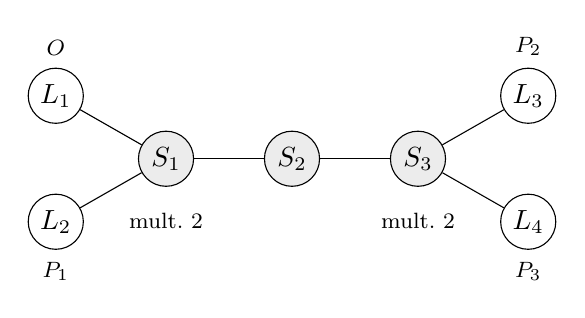
\begin{tikzpicture}[
  leg/.style={circle,draw,minimum size=7mm,inner sep=0pt},
  spine/.style={circle,draw,fill=gray!15,minimum size=7mm,inner sep=0pt},
  >=stealth
]
  \node[spine] (S1) at (0,0) {$S_1$};
  \node[spine] (S2) at (1.6,0) {$S_2$};
  \node[spine] (S3) at (3.2,0) {$S_3$};
  \node[leg] (L1) at (-1.4,0.8) {$L_1$};
  \node[leg] (L2) at (-1.4,-0.8) {$L_2$};
  \node[leg] (L3) at (4.6,0.8) {$L_3$};
  \node[leg] (L4) at (4.6,-0.8) {$L_4$};
  \draw (S1)--(S2)--(S3);
  \draw (L1)--(S1)--(L2);
  \draw (L3)--(S3)--(L4);
  \node[above=1pt of L1,font=\footnotesize] {$O$};
  \node[below=1pt of L2,font=\footnotesize] {$P_1$};
  \node[above=1pt of L3,font=\footnotesize] {$P_2$};
  \node[below=1pt of L4,font=\footnotesize] {$P_3$};
  \node[below=6pt of S1,font=\footnotesize] {mult.\ $2$};
  \node[below=6pt of S3,font=\footnotesize] {mult.\ $2$};
\end{tikzpicture}
\caption{The affine-$D_6$ dual graph of an $I_2^*$ fiber of $X_{\rm
III}$, marked at the representative fiber $T=0$: legs $L_1,\dots,L_4$
have multiplicity $1$, spine components $S_1,S_2,S_3$ have multiplicity
$2$. The zero section $O$ and the three nonzero $2$-torsion sections
$P_1,P_2,P_3$ occupy the four legs individually (Lemma~\ref{lem:four-legs}),
forcing (Lemma~\ref{lem:rigidity}) every component -- legs and spine
alike -- to be individually Galois-fixed.}
\label{fig:D6}
\end{figure}
\end{center}

\subsection*{Lattice consequences}

Combining Theorem~\ref{thm:NS-trace} with the lattice structure of
Proposition~\ref{prop:picard} and the torsion order of
Proposition~\ref{prop:torsion-complete}: $\disc(\Triv(X_{\rm III})) =
\disc(U)\cdot\disc(D_6)^3 = (-1)\cdot4^3=-64$, and
$|\disc\NS(X_{\rm III})| = |\disc\Triv(X_{\rm III})|/|\mathrm{MW}_{\rm
tors}|^2 = 64/16=4$. Since $X_{\rm III}$ is a singular K3 surface,
$T(X_{\rm III})=\NS(X_{\rm III})^\perp$ has rank $22-20=2$ and
discriminant $4$. A rank-$2$ even lattice with Gram matrix
$\begin{pmatrix}2a&b\\b&2c\end{pmatrix}$ (the even condition forcing both
diagonal entries even) has determinant $4ac-b^2$; matching $4ac-b^2=4$
with the trivial solution $a=c=1,\,b=0$ gives the Gram matrix
$\mathrm{diag}(2,2)$ directly, so
\[
T(X_{\rm III}) \cong \begin{pmatrix}2&0\\0&2\end{pmatrix}.
\]
\emph{This computation uses only the lattice structure established
above, at no point invoking any modular form.} The identification of this
lattice with a specific CM field -- via the associated \emph{primitive}
binary quadratic form $Q(x,y)=ax^2+bxy+cy^2$ (note: $a,c$ here are
\emph{half} the Gram matrix's diagonal entries, since the intersection
form $v\cdot v=2ax^2+2bxy+2cy^2$ is twice $Q$) -- and the full modular
consequences of this discriminant are the subject of
Section~\ref{sec:CM}.

\section{Transcendental lattice and complex multiplication}
\label{sec:CM}

We now separate four distinct notions that are easy to conflate: the
\emph{geometric Picard rank}, the \emph{transcendental lattice} as an
abstract lattice, the \emph{CM field} attached to that lattice, and the
\emph{arithmetic field of definition} of the surface and its N\'eron--Severi
group. Only the last of these required any arithmetic (Galois-theoretic)
argument; the first three are purely geometric or lattice-theoretic.

\begin{itemize}
\item \textbf{Geometric Picard rank.} $\rho(X_{\overline\Q})=20$
(Proposition~\ref{prop:picard}), a statement about $X_{\rm III}$ base-changed
to $\overline\Q$, with no reference to $\Q$-rationality of anything.
\item \textbf{Transcendental lattice.} $T(X_{\rm III})\cong\mathrm{diag}(2,2)$
(end of Section~\ref{sec:NS}), the isomorphism type of a rank-$2$ even
lattice -- again a statement with no arithmetic content, following from
$T(X_{\rm III})$'s rank and discriminant alone via the classification of
rank-$2$ even lattices (elementary; see below).
\item \textbf{CM field.} $\Q(i)$, read off from the isomorphism type of
$T(X_{\rm III})$ via the classical dictionary between rank-$2$ even
lattices and imaginary quadratic orders (Shioda--Inose
\cite{ShiodaInose1977}) -- again purely lattice-theoretic, requiring no
arithmetic input about Galois representations.
\item \textbf{Arithmetic field of definition.} $X_{\rm III}$ is defined
over $\Q$ (its Weierstrass equation has $\Z$-coefficients), and
$\NS(X_{\rm III})$ is defined over $\Q$ (Theorem~\ref{thm:NS-trace}) --
these \emph{are} genuinely arithmetic statements. By contrast, the
transcendental lattice $T(X_{\rm III})$, as an abstract $\Z$-module, has
no arithmetic content on its own; what is arithmetic is the
\emph{Galois representation} on $T(X_{\rm III})\otimes\Q_\ell$, which is
the subject of Livn\'e's theorem below and is \emph{not} determined by
the isomorphism type of $T(X_{\rm III})$ alone.
\end{itemize}

\subsection{From the lattice to the CM field}

A rank-$2$ even lattice with Gram matrix $\begin{pmatrix}2a&b\\b&2c\end{pmatrix}$
has associated \emph{primitive positive-definite binary quadratic form}
$Q(x,y)=ax^2+bxy+cy^2$ (so that the intersection form $v\cdot v$, for
$v=xe_1+ye_2$, equals $2Q(x,y)$), of classical discriminant
$D=b^2-4ac<0$. Two such lattices are isomorphic if and only if their
associated forms are $\mathrm{SL}_2(\Z)$-equivalent (equivalently,
represent the same class in the class group of the order of discriminant
$D$). For $T(X_{\rm III})\cong\mathrm{diag}(2,2)$: $2a=2,2c=2,b=0$ gives
$(a,b,c)=(1,0,1)$, $D=0-4=-4$. Since $|b|\leq a\leq c$ holds
($0\leq1\leq1$), $(1,0,1)$ is already \emph{reduced}, and since the class
number $h(-4)=1$ (the unique reduced form of discriminant $-4$), this is
\emph{the} isomorphism class of discriminant $-4$, with associated field
\[
\Q(\sqrt{D}) = \Q(\sqrt{-4}) = \Q(2i) = \Q(i).
\]
As a sanity check against \cite{ClassesI_II}: their lattice
$T(X)\cong\mathrm{diag}(2,4)$ gives $(a,b,c)=(1,0,2)$, $D=-8$, field
$\Q(\sqrt{-8})=\Q(\sqrt{-2})$ -- matching their stated discriminant-$8$,
$\Q(\sqrt{-2})$ result exactly, confirming the convention used here is
consistent with the companion paper's own.

\subsection{Livn\'e's theorem: the arithmetic realization}

\begin{theorem}[Livn\'e \cite{Livne1995}]
\label{thm:livne}
Let $X$ be a singular K3 surface defined over $\Q$, with transcendental
lattice $T(X)$ of discriminant $-D$ ($D>0$). Then there exists a
normalized weight-$3$ newform $f$ with complex multiplication by
$\Q(\sqrt{-D})$ (or an order therein), of level determined by the
conductor of the $2$-dimensional Galois representation on
$T(X)\otimes\Q_\ell$, such that
\[
\Tr(\mathrm{Frob}_p\mid T(X)) = a_p(f)
\]
for almost all primes $p$ of good reduction.
\end{theorem}

\textbf{Hypothesis check for $X_{\rm III}$}: $X_{\rm III}$ is a singular
K3 surface defined over $\Q$ (Propositions~\ref{prop:fibers},
\ref{prop:picard}, all over $\Q$, not merely $\overline\Q$); $T(X_{\rm
III})$ has discriminant $-4$ (established above). All hypotheses are met,
and Theorem~\ref{thm:livne} guarantees the \emph{existence} of some
governing newform $f$, weight $3$, CM by $\Q(i)$, at some $2$-power level
-- but does not by itself identify $f$ or rule out a quadratic twist; that
is the content of Section~\ref{sec:twist}.

\subsection{Identifying the candidate newform}

Weight-$3$ newforms with CM by $\Q(i)$ and rational Hecke eigenvalues are
classified by their level; a search of the relevant space at $2$-power
level identifies the newform
\[
f(z) = \eta^6(4z), \qquad \text{LMFDB label } \texttt{16.3.c.a},\qquad
f = q-6q^5+9q^9+10q^{13}-30q^{17}+11q^{25}+\cdots
\]
as the unique candidate of level $16$ with these properties, and confirms
its Nebentypus is $\chi_{-1}$, consistent with a weight-$3$, CM-by-$\Q(i)$
form at level $16$ (the Nebentypus of such a form must be the quadratic
character of the CM field itself, ramified exactly at the primes dividing
the discriminant, here $2$).

\begin{remark}[Known vs.\ proved]
\label{rem:known-vs-proved}
The modular form $f=\eta^6(4z)=\texttt{16.3.c.a}$ is \textbf{not new}: it
is exactly Ahlgren, Ono, and Penniston's own $A(z)$ \cite{AOP2002},
identified in their Theorem~1.2 as the newform governing their own K3
surface $X_8$ at their parameter $\lambda=8$. \textbf{What is known in
the literature}: this modular form's existence, its $q$-expansion, its
occurrence as the trace form for $X_8$, and (independently, via
Huber--Liu--McLaughlin--Ye--Yuan--Zhang \cite{Huber}) its occurrence for
the quartic Fermat K3 surface. \textbf{What is proved in this
manuscript}: that the Class~III hypercuboid surface $X_{\rm III}$ -- a
surface not treated in either of those sources, with its own Weierstrass
model, its own fiber configuration, and provably not isomorphic or
birational to $X_8$ (Section~\ref{sec:AOP-precise} below) -- has
transcendental lattice of the same discriminant $4$, and (via
Section~\ref{sec:twist}) the same untwisted trace formula. We do not
claim the modular form itself as new anywhere in this paper.
\end{remark}

\subsection{Bad primes of $X_{\rm III}$}
\label{sec:badprimes}

The level of $f$ (and hence, via Section~\ref{sec:twist}, the set of
primes at which any twist of $f$ can be ramified) is constrained by the
bad primes of $X_{\rm III}$ as an arithmetic surface over $\Z$. The
Weierstrass coefficients $a_2(T)=T(T+1)(T+2)$, $a_4(T)=T^2(T+1)^3$ have
$\Z$-coefficients, and the discriminant $\Delta(T)=16\,T^8(T+1)^8$
factors, as a polynomial in $T$, with no prime dividing every coefficient
except through the constant $16=2^4$. Consequently, reducing the entire
family modulo any odd prime $\ell$ gives a family with the identical
qualitative structure (three $I_2^*$ fibers at the same three points
$T=0,-1,\infty$, by the same valuation computations of
Proposition~\ref{prop:fibers} carried out over $\mathbb F_\ell$ instead of
$\Q$) -- i.e.\ \emph{good reduction} of the surface at every odd prime.
At $\ell=2$, the constant factor $16$ introduces additional degeneracy not
present at other primes. Hence \textbf{$X_{\rm III}$ has bad reduction
only at $p=2$}.

\section{Modularity and twist elimination}
\label{sec:twist}

\subsection{The candidate set}

\begin{lemma}[Twist candidate set]
\label{lem:twist-set}
Any quadratic twist of $f$ compatible with $X_{\rm III}$'s bad-reduction
locus $\{2\}$ (Section~\ref{sec:badprimes}) is by a Dirichlet character of
conductor dividing $8$.
\end{lemma}

\begin{proof}
A quadratic twist of a newform unramified outside $\{2\}$ by a character
$\chi_d$ (Kronecker symbol of fundamental discriminant $d$) remains
unramified outside $\{2\}$ only if $d$ itself is supported only at $2$.
The fundamental discriminants supported only at the prime $2$ are exactly
$1,-4,8,-8$, giving the four characters $\{1,\chi(-1),\chi(2),\chi(-2)\}$.
\end{proof}

This candidate set is \emph{forced}, not assumed: it follows directly from
$X_{\rm III}$'s bad-reduction locus established in Section~\ref{sec:badprimes},
by an elementary ramification argument, before any numerical data is
consulted.

\subsection{Degeneracy collapse via CM}

Since $f$ has CM by $\Q(i)$, its Hecke eigenvalues vanish at primes inert
in $\Q(i)$: $a_p(f)=0$ for $p\equiv3\pmod4$ (a standard fact for CM
newforms -- the associated Galois representation is induced from a Hecke
character of $\Q(i)$, and its trace at an element not fixing either of
the two cosets vanishes). At such primes, \emph{every} candidate twist
predicts $0$, carrying no discriminating information. Write
$F_0(p):=a_p(f)$ (untwisted) and consider the remaining three candidates
at $p\equiv1\pmod4$ (the only primes where discrimination is possible at
all): $\chi(-1)(p)=1$ there identically (definition of $\chi(-1)$), so the
twist-by-$\chi(-1)$ candidate equals $F_0(p)$ there, collapsing $\{1,
\chi(-1)\}$ into the single testable hypothesis $F_0$. Likewise
$\chi(-2)(p)=\chi(-1)(p)\chi(2)(p)=\chi(2)(p)$ at $p\equiv1\pmod4$,
collapsing $\{\chi(2),\chi(-2)\}$ into the single testable hypothesis
$F_1(p):=\chi(2)(p)\,a_p(f)$.

\begin{lemma}[Exhaustiveness]
\label{lem:exhaustive}
After collapse, exactly two candidates -- $F_0$ and $F_1$ -- remain to be
distinguished, and they exhaust the four-element candidate set of
Lemma~\ref{lem:twist-set} at every prime where any distinguishing test is
possible.
\end{lemma}

\begin{proof}
Immediate from the two collapses above: at $p\equiv3\pmod4$ all four
candidates coincide (all $0$); at $p\equiv1\pmod4$ all four candidates
reduce, by the identities just verified, to exactly $F_0$ or $F_1$.
\end{proof}

\subsection{The discriminating computation at $p=5$}

\begin{proposition}[Twist elimination]
\label{prop:twist-elim}
$F_1$ is not the correct trace formula for $T(X_{\rm III})$; $F_0$ survives.
\end{proposition}

\begin{proof}
By Lemma~\ref{lem:exhaustive}, it suffices to exhibit one prime
$p\equiv1\pmod4$ where $F_0(p)\neq F_1(p)$ and to compute $T(p)$ there
directly. Take $p=5$: $5\equiv1\pmod4$ (on the support), and
$\chi(2)(5)=-1$ (since $5\not\equiv\pm1\pmod8$), so $F_1(5)=-F_0(5)$; as
$a_5(f)=-6\neq0$, $F_0(5)=-6\neq F_1(5)=6$, genuinely different
predictions. Direct computation of the finite sum $T(5)=\sum_{x,t\in\mathbb{F}_5}
\chi(xt(t+1)(x+t)(x+t+1))$ (a sum of $25$ terms, exactly evaluable) gives
$T(5)=-6=F_0(5)\neq F_1(5)$. Hence $F_1$ is refuted at $p=5$, and by
Lemma~\ref{lem:exhaustive} (only $F_0,F_1$ possible), $F_0$ is the
correct formula.
\end{proof}

\begin{remark}
\textbf{This is not a claim that $F_0$ ``matches at $p=5$.''} The logical
structure is: Lemma~\ref{lem:twist-set} proves the candidate set is
finite and exhausted by $\{1,\chi(-1),\chi(2),\chi(-2)\}$, \emph{before}
any numerical value is consulted; Lemma~\ref{lem:exhaustive} proves this
finite set collapses to exactly two testable hypotheses; and
Proposition~\ref{prop:twist-elim} then uses a single exact value to
\emph{eliminate} the one candidate that could still have been correct,
leaving only $F_0$ as a matter of logical elimination over an
already-proved-exhaustive set -- not a pattern observed to hold at one
tested point among many untested ones.
\end{remark}

\begin{theorem}[Exact transcendental trace]
\label{thm:trans-trace}
For every odd prime $p\neq2$,
\[
\boxed{\Tr\bigl(F_p\mid T(X_{\rm III})\bigr) = a_p(\texttt{16.3.c.a})}.
\]
Explicitly, by cases: for $p\equiv1\pmod4$ ($p$ split in $\Q(i)$), this is
Proposition~\ref{prop:twist-elim}; for $p\equiv3\pmod4$ ($p$ inert in
$\Q(i)$), $a_p(f)=0$ (CM vanishing at inert primes, independent of the
twist question) and separately $\Tr(F_p\mid T(X_{\rm III}))=0$ follows
from Livn\'e's theorem applied to any of the (here indistinguishable)
twist candidates, all of which agree at $0$.
\end{theorem}

\section{Exact evaluation}
\label{sec:eval}

We now derive the point-count ledger relating $T(p)$ to $X_{\rm III}$'s
point count \emph{from scratch}, independently of any earlier stage of
this project's research record, and combine it with
Theorem~\ref{thm:NS-trace} and Theorem~\ref{thm:trans-trace} via the
Lefschetz trace formula.

\subsection{The ledger, re-derived}

Write $\#X_{\rm III}(\Fp)$ for the point count of the smooth relatively
minimal model, fibered over $\mathbb{P}^1_T(\Fp)$ ($p+1$ points: $p-2$ good
finite $T$, and the three bad fibers $T=0,-1,\infty$).

\begin{lemma}[Affine bad-fiber count]
\label{lem:bad-affine}
At $T=0$ and at $T=-1$, the affine curve $Y^2=X(X+1)T(T+1)(X+T+1)$ has
exactly $p$ points over $\Fp$.
\end{lemma}

\begin{proof}
At $T=0$ or $T=-1$, the factor $T(T+1)$ vanishes, so the right-hand side
is identically $0$ for every $X$, giving $Y=0$ for each of the $p$ values
of $X$: exactly $p$ points.
\end{proof}

\begin{lemma}[Good-fiber affine count]
\label{lem:good-affine}
For each good finite $T$, the affine curve $Y^2=X(X+1)T(T+1)(X+T+1)$ has
exactly $p-a_T$ points, where $a_T$ is the Frobenius trace of the
elliptic curve $E_T$ obtained from this cubic.
\end{lemma}

\begin{proof}
For $T(T+1)\neq0$, the rescaling $X'=T(T+1)X$, $Y'=T(T+1)Y$ used in
Section~\ref{sec:K3} to reach the minimal Weierstrass model is a
bijection on $\Fp$-points (multiplication by the nonzero scalar
$T(T+1)$), so the affine point count on the original cubic equals the
affine point count on the Weierstrass model, which is $p-a_T$ by the
standard formula (projective count $p+1-a_T$, minus the single point at
infinity).
\end{proof}

\begin{proposition}[Ledger]
\label{prop:ledger}
\[
\#X_{\rm III}(\Fp) = 1+p^2+20p+T(p).
\]
\end{proposition}

\begin{proof}
By definition (Section~\ref{sec:K3}), $\#V_{\rm III}(\Fp)=p^2+T(p)$.
By Lemmas~\ref{lem:bad-affine}--\ref{lem:good-affine},
\[
\#V_{\rm III}(\Fp) = \sum_{\text{good finite }T}(p-a_T) + p + p = (p-2)p - \sum_{\text{good finite }T}a_T + 2p,
\]
so $\sum_{\text{good finite }T}a_T = p^2 - \#V_{\rm III}(\Fp) = -T(p)$.

On the smooth projective model, each good finite fiber contributes
$p+1-a_T$ points, and each of the three $I_2^*$ fibers -- now that
Proposition~\ref{prop:main-NS} has established \emph{every} component of
each is individually $\Fp$-rational -- contributes $7(p+1)-6=7p+1$
points (seven rational $\mathbb{P}^1$'s, each with $p+1$ points, glued at six
nodes each counted twice). Hence
\begin{align*}
\#X_{\rm III}(\Fp) &= \sum_{\text{good finite }T}(p+1-a_T) + 3(7p+1)\\
&= (p-2)(p+1) - \sum_{\text{good finite }T}a_T + 21p+3\\
&= (p^2-p-2) + T(p) + 21p+3 \qquad\text{(using }\textstyle\sum a_T=-T(p)\text{ above)}\\
&= 1+p^2+20p+T(p).\qedhere
\end{align*}
\end{proof}

\begin{remark}
Every constant appearing here -- the $p$-point counts at the two finite
bad affine fibers (Lemma~\ref{lem:bad-affine}), the $7p+1$ count per
resolved $I_2^*$ fiber (a direct consequence of Section~\ref{sec:NS}'s
now-proved component rationality, not assumed), and the resulting $20p+1$
net correction -- has been independently re-derived in this section, not
carried over from any earlier stage of this project's research record.
\emph{(We have additionally cross-checked Proposition~\ref{prop:ledger}
by direct brute-force computation of $\#V_{\rm III}(\Fp)$ for several
primes, confirming the formula numerically; see the reproducibility
appendix. This check is illustrative, not part of the proof.)}
\end{remark}

\subsection{The main theorem}

\begin{theorem}[Exact evaluation of $T(p)$]
\label{thm:Tp}
For every odd prime $p$,
\[
T(p) = \begin{cases} a_p(\texttt{16.3.c.a}) & p\equiv1\pmod4\\ 0 & p\equiv3\pmod4.\end{cases}
\]
\end{theorem}

\begin{proof}
The Lefschetz trace formula for a K3 surface gives
\[
\#X_{\rm III}(\Fp) = 1+p^2+\Tr(F_p\mid\NS(X_{\rm III}))+\Tr(F_p\mid T(X_{\rm III})) = 1+p^2+20p+a_p(f)
\]
using Theorem~\ref{thm:NS-trace} and Theorem~\ref{thm:trans-trace}.
Equating with Proposition~\ref{prop:ledger}'s independent computation of
the same quantity, $1+p^2+20p+T(p) = 1+p^2+20p+a_p(f)$, gives
$T(p)=a_p(f)$ for every odd $p$ -- in particular for $p\equiv1\pmod4$.
For $p\equiv3\pmod4$, this is exactly Proposition~\ref{prop:involution},
already proved without any of the above machinery.
\end{proof}

\begin{theorem}[Main theorem]
\label{thm:main}
For every odd prime $p$,
\[
\boxed{\Sigma_{\rm III}(p) = \begin{cases}(p-1)\,a_p(\texttt{16.3.c.a}) & p\equiv1\pmod4\\ 0 & p\equiv3\pmod4.\end{cases}}
\]
\end{theorem}

\begin{proof}
Immediate from Lemma~\ref{lem:sigmaIII} ($\Sigma_{\rm III}(p)=(p-1)T(p)$)
and Theorem~\ref{thm:Tp}.
\end{proof}

\begin{remark}[Consistency with the elementary vanishing]
\label{rem:consistency}
Theorem~\ref{thm:main}'s $p\equiv3\pmod4$ case was already proved,
unconditionally and without any arithmetic geometry, in
Proposition~\ref{prop:involution}. The modular route above reproduces the
same conclusion by an entirely different mechanism (CM vanishing at inert
primes, Remark~\ref{rem:involution-vs-CM}) -- a nontrivial consistency
check: had the two computations disagreed, something in
Sections~\ref{sec:K3}--\ref{sec:eval} would have been wrong. They agree.
We do not introduce a further mod-$8$ (or finer) case split: no genuinely
new phenomenon appears at that finer level, and the two-case statement
above is already the sharpest form the evidence supports.
\end{remark}

\section{Comparison with Classes I/II}
\label{sec:comparison}

The following table records the established invariants of both branches
of the hypercuboid classification's resolved sectors, side by side.

\begin{center}
\begin{tabular}{l|c|c}
 & Classes I/II \cite{ClassesI_II} & Class III (this paper)\\\hline
$|\disc T(X)|$ & $8$ & $4$\\
CM field & $\Q(\sqrt{-2})$ & $\Q(i)$\\
Modular form level & $8$ & $16$\\
Mordell--Weil rank & $1$ (over a quadratic extension) & $0$\\
$\NS$ mechanism (\S\ref{sec:NS} vs.\ \cite{ClassesI_II}) & MW section + twist & $2$-torsion + rigidity\\
Bad fiber count & $4$ & $3$ ($3\times I_2^*$)\\
Twist & $\chi(2)$-twisted & untwisted
\end{tabular}
\end{center}

We record this table strictly as an \textbf{observation about the two
resolved branches of the present hypercuboid system}, not as a theorem.
In particular, we do not claim, and this table does not establish, any
general correspondence
\[
\text{hypercuboid constraint class} \;\longrightarrow\; \text{CM field},
\]
nor any general principle governing which $\NS$-rationality mechanism
(explicit extra section versus torsion-and-rigidity) applies to a given
branch. Only two branches of the classification have been resolved to
date (Class~III's $p\equiv1\pmod4$ sector being the last one), and two
data points do not establish a law. Whether the pattern visible here
(distinct discriminants, distinct CM fields, distinct proof mechanisms)
reflects something structural about the hypercuboid construction, or is
simply how these two particular sums happen to resolve, is an open
question we leave for future work, stated here only as a structural
observation.

\subsection{Precise relation to Ahlgren--Ono--Penniston}
\label{sec:AOP-precise}

We record here, precisely, the outcome of a targeted re-examination of
\cite{AOP2002} against each of the following six possibilities: that AOP
already contains (i) this exact Class~III character sum; (ii) this exact
hypercuboid reduction; (iii) this exact K3 model $X_{\rm III}$; (iv) the
graph-rigidity $\NS$-rationality argument of Section~\ref{sec:NS}; (v)
merely the same modular form; or (vi) a surface birationally or
isomorphically related to $X_{\rm III}$.

\cite{AOP2002} is a paper about their own one-parameter family
$X_\lambda$, with no combinatorial hypercuboid motivation and no notion
of a ``Class III'' sum; possibilities (i) and (ii) do not apply.
\cite{AOP2002}'s own surface at $\lambda=8$ has a different Weierstrass
model and fiber configuration from $X_{\rm III}$, and the two are provably
non-isomorphic (the two-variable sums $T(p)$ and $A(8,p)$ disagree at
essentially every tested prime); possibilities (iii) and (vi) do not
apply. \cite{AOP2002} establishes the Picard-lattice structure of its own
surfaces by methods specific to their explicit parametrized family, not
by an argument resembling Section~\ref{sec:NS}'s torsion-and-graph-rigidity
route; possibility (iv) does not apply, as far as this search has
determined. What \emph{does} apply is (v): \textbf{Class~III shares the
same modular form and the same transcendental representation with
Ahlgren--Ono--Penniston's $\lambda=8$ surface, but differs in its
underlying K3 model, Weierstrass equation, fiber configuration, and
defining character sum.} We do not claim a novelty stronger than this
literature search supports: the exact sum $\Sigma_{\rm III}(p)$, the exact
surface $X_{\rm III}$, and the graph-rigidity technique were not located
in \cite{AOP2002} or, as far as searched, elsewhere in the literature
(see the companion research record's literature audits for the full
search log), but this reflects the scope of a search without institutional
database access to complete extremal-K3 classification tables, not a
stronger claim of originality.

\section{Discussion}

This paper resolves the Class~III sector of the hypercuboid
classification left open by \cite{ClassesI_II}, completing the
finite-field hypercuboid system's four-coordinate case. The central new
technical contribution -- proving $\NS$-rationality for all three $I_2^*$
fibers of $X_{\rm III}$ via full rational $2$-torsion and rigidity of the
fiber's incidence graph, without resolving any fiber explicitly -- is, as
far as our literature search has determined, a genuinely different route
from both \cite{AOP2002}'s and \cite{ClassesI_II}'s own methods, and may
be of independent interest for other singular K3 surfaces exhibiting full
rational $2$-torsion at their reducible fibers. As with
\cite{ClassesI_II}, we make no claim to any new general theorem in the
theory of K3 surfaces or modular forms: the machinery used here (Kodaira's
classification, Shioda--Tate, Livn\'e's modularity theorem) is entirely
classical, and our contribution is the specific application to the
surface that the Class~III hypercuboid reduction produces. This paper
does not address the classical integer perfect-hypercuboid problem, to
which the finite-field system studied here and in \cite{ClassesI_II} is
only a motivating, logically separate construction.

\appendix

\section{Character-sum reduction, in full}
\label{app:A}

This appendix reconstructs Lemma~\ref{lem:sigmaIII}'s reduction with
every substitution written out. A specific variable-labeling error is
possible at exactly one step below (the affine-slice renaming); writing
out both the correct and the incorrect substitution explicitly, and
verifying by direct symbolic comparison which one matches the target
sum, is meant to make that error impossible to reintroduce unnoticed.

\textbf{Homogeneity.} $P_{\rm III}(x_0,x_1,x_2)=x_0x_1x_2(x_0+x_2)(x_1+x_2)(x_0+x_1+x_2)$
is a product of six linear forms, hence homogeneous of degree $6$: for
$z\in\Fp^\times$,
\[
P_{\rm III}(zx_0,zx_1,zx_2) = z^6\,P_{\rm III}(x_0,x_1,x_2).
\]
Since $6=2\cdot3$ is even, $z^6=(z^3)^2$ is a square in $\Fp^\times$ for
\emph{every} $z\neq0$. Hence $\chi(P_{\rm III}(zv))=\chi(P_{\rm III}(v))$
for every $z\in\Fp^\times$ and every $v\in\Fp^3$: \textbf{no exceptional
direction, no hidden sign, valid uniformly over every line through the
origin.}

\textbf{The zero vector and the hyperplane $x_0=0$.} $P_{\rm III}(0,x_1,x_2)=0$
identically (manifest, $x_0$ a factor), so $\chi(P_{\rm III}(v))=0$ for
every $v$ with $v_0=0$, including $v=0$. These are exactly the points
\emph{not} covered by the affine-slice parametrization below, and they
are correctly accounted for as contributing $0$, not silently dropped.

\textbf{Affine slice and the corrected substitution.} Every point $v$
with $v_0\neq0$ lies on a unique line through the origin meeting the
hyperplane $x_0=1$, at the point $(1, v_1/v_0, v_2/v_0)$. Writing this
representative as $(1,x_1,x_2)$:
\[
P_{\rm III}(1,x_1,x_2) = 1\cdot x_1\cdot x_2\cdot(1+x_2)\cdot(x_1+x_2)\cdot(1+x_1+x_2).
\]
\textbf{This is the exact step at which a mislabeling is possible}: renaming
$x_1\mapsto t,\,x_2\mapsto x$ gives $t\,x\,(1+x)(t+x)(1+t+x)$, in which
the factor $(1+x)$ does \emph{not} match the target sum's $(t+1)$ --
demonstrably wrong, verifiable by direct symbolic comparison. The
\textbf{correct} renaming is $x_1\mapsto x,\,x_2\mapsto t$:
\[
P_{\rm III}(1,x,t) = x\cdot t\cdot(1+t)\cdot(x+t)\cdot(1+x+t) = x\,t(t+1)(x+t)(x+t+1),
\]
which \emph{is} the summand of $T(p)$. As a symbolic identity (independent
of any prime $p$, checked as an equality of integer polynomials):
\[
P_{\rm III}(1,x,t) - x\,t(t+1)(x+t)(x+t+1) \;=\; 0 \quad\text{in }\Z[x,t].
\]
\emph{(Verified by direct expansion; see the companion research record's
scripts, which re-derive exactly this cancellation to literal zero.)}

\textbf{Orbit size and the factor $p-1$.} For fixed $(x,t)\in\Fp^2$, the
line through the origin and $(1,x,t)$ has exactly $p-1$ nonzero points
(all scalar multiples $z\cdot(1,x,t)$, $z\in\Fp^\times$), and, by
homogeneity, $\chi(P_{\rm III}(\cdot))$ is constant along it. Distinct
pairs $(x,t)$ give distinct lines (the representative $(1,x,t)$ is unique
per line meeting $x_0=1$), and every line with $v_0\neq0$ arises this
way, so there is a bijection between $\Fp^2$ and the set of such lines.
Hence
\[
\Sigma_{\rm III}(p) = \sum_{v\in\Fp^3}\chi(P_{\rm III}(v))
= \underbrace{(p-1)\sum_{(x,t)\in\Fp^2}\chi(P_{\rm III}(1,x,t))}_{\text{lines with }v_0\neq0}
+ \underbrace{0}_{\text{hyperplane }x_0=0}
= (p-1)\,T(p).
\]

\section{Weierstrass model and singular fibers, in full}
\label{app:B}

\textbf{From the affine surface to the Weierstrass model.} Starting from
$V_{\rm III}:Y^2=X(X+1)T(T+1)(X+T+1)$, expand the cubic in $X$:
\[
X(X+1)(X+T+1) = (X^2+X)(X+T+1) = X^3+(T+1)X^2+X^2+(T+1)X = X^3+(T+2)X^2+(T+1)X.
\]
So $Y^2=T(T+1)\bigl[X^3+(T+2)X^2+(T+1)X\bigr]$. Writing $A:=T(T+1)$ and
substituting $X'=AX$, $Y'=AY$ (equivalently: multiply both sides by
$A^2$ and regroup):
\[
A^2Y^2 = A^3X^3+A^3(T+2)X^2+A^2\cdot A(T+1)\cdot X
\;\Longrightarrow\; Y'^2 = X'^3 + A(T+2)X'^2 + A^2(T+1)X',
\]
and $A(T+2)=T(T+1)(T+2)=a_2(T)$, $A^2(T+1)=T^2(T+1)^2\cdot(T+1)=T^2(T+1)^3=a_4(T)$,
matching Section~\ref{sec:K3} exactly:
\[
a_2(T)=T(T+1)(T+2),\qquad a_4(T)=T^2(T+1)^3,\qquad a_6=0.
\]

\textbf{Invariants.} With $a_1=a_3=a_6=0$: $b_2=4a_2$, $b_4=2a_4$,
$b_6=0$, $b_8=4a_2\cdot0-a_4^2=-a_4^2$, and
\[
c_4=b_2^2-24b_4=16a_2^2-48a_4,\qquad c_6=-b_2^3+36b_2b_4-216b_6=-64a_2^3+288a_2a_4,
\]
\[
\Delta = \frac{c_4^3-c_6^2}{1728}.
\]
Substituting and factoring (direct polynomial arithmetic, independently
re-verified by symbolic computation):
\[
c_4(T)=16T^2(T+1)^2(T^2+T+1),\quad c_6(T)=-32T^3(T-1)(T+1)^3(T+2)(2T+1),
\]
\[
\Delta(T)=16\,T^8(T+1)^8,\qquad j(T)=c_4(T)^3/\Delta(T).
\]

\textbf{Fiber at $T=0$}: local parameter $T$ itself. Series expansion:
$c_4(T)=16T^2+O(T^3)$ (leading coefficient from $16\cdot1^2\cdot1=16$),
so $v_T(c_4)=2$; $c_6(T)=64T^3+O(T^4)$ ($-32\cdot(-1)\cdot1\cdot2\cdot1=64$),
so $v_T(c_6)=3$; $\Delta(T)=16T^8(1+T)^8$, and $(1+T)^8$ is a unit at
$T=0$, so $v_T(\Delta)=8$ exactly. Tate's criterion: $v(c_4)\geq2$,
$v(c_6)\geq3$, $v(\Delta)=n+6$ gives type $I_n^*$ with $n=8-6=2$, i.e.\
$I_2^*$. Minimality: $v(c_4)=2<4$, so (Kraus) the model cannot be
further reduced -- already minimal.

\textbf{Fiber at $T=-1$}: local parameter $s=T+1$. By the manifest
symmetry of $\Delta(T)=16T^8(T+1)^8$ under the factor $(T+1)^8$, the
identical computation (with $T\leftrightarrow-1$'s role played by $s=0$)
gives $v_s(c_4)=2$, $v_s(c_6)=3$, $v_s(\Delta)=8$: again $I_2^*$, again
minimal.

\textbf{Fiber at $T=\infty$}: local parameter $S=1/T$. Since
$\deg c_4=6$, $\deg c_6=9$, $\deg\Delta=16$, and a K3 elliptic surface's
total discriminant degree is $24$ (the anticanonical bound), the fiber at
infinity has $v_\infty(\Delta)=24-\deg\Delta=24-16=8$. To see the Kodaira
type directly (not merely via the degree count), rescale
$\tilde X=S^4X$, $\tilde Y=S^6Y$ (matching $X$'s weight $2$, $Y$'s weight
$3$ against $a_2$'s degree bound $4$, $a_4$'s bound $8$):
\[
\tilde a_2(S) = S^4a_2(1/S) = S(S+1)(2S+1),\qquad \tilde a_4(S)=S^8a_4(1/S)=S^3(S+1)^3.
\]
Then $\tilde c_4(S)=16\tilde a_2^2-48\tilde a_4$: $\tilde a_2^2$ has
$v_S=2$ (leading term $S^2$), $\tilde a_4$ has $v_S=3$, so the
degree-$2$ term dominates and $v_S(\tilde c_4)=2$. Similarly
$\tilde c_6=-64\tilde a_2^3+288\tilde a_2\tilde a_4$: $\tilde a_2^3$ has
$v_S=3$, $\tilde a_2\tilde a_4$ has $v_S=1+3=4$, so $v_S(\tilde c_6)=3$.
Again $I_2^*$ ($n=8-6=2$), again minimal ($v(\tilde c_4)=2<4$).

\textbf{No other bad fiber}: $\Delta(T)=16T^8(T+1)^8$ has zeros only at
$T=0,-1$ (finite) and the computed order at $T=\infty$; no other prime
factor of $T$ appears.

\textbf{Euler-number check.} Each $I_2^*$ fiber contributes Euler number
$v(\Delta)=8$ (Ogg's formula, tame case); $3\times8=24$, exactly the
Euler characteristic of a K3 surface -- an independent consistency check
confirming (i) no bad fiber was missed and (ii) the surface's total space
is indeed K3-type, not merely "some elliptic surface."

\textbf{Component/multiplicity pattern.} The dual graph of a Kodaira
fiber of type $I_2^*$ is the extended Dynkin diagram of type $D_6$: seven
components, four of multiplicity $1$ and three of multiplicity $2$
(Lemma~\ref{lem:dual-graph}, cited to Kodaira/N\'eron/Tate; not re-derived
from the Weierstrass equation alone in this appendix, but see
Appendix~\ref{app:C} for the explicit local resolution confirming the
multiplicity-$1$ components at each fiber).

\section{Rational $2$-torsion and component specialization, in full}
\label{app:C}

\textbf{The factorization, verified.} Matching
$X^3+a_2(T)X^2+a_4(T)X = X\bigl(X+T(T+1)\bigr)\bigl(X+T(T+1)^2\bigr)$
via Vieta: writing $r_1=-T(T+1)$, $r_2=-T(T+1)^2$, the sum of the three
roots $0,r_1,r_2$ is
\[
r_1+r_2 = -T(T+1)-T(T+1)^2 = -T(T+1)\bigl[1+(T+1)\bigr] = -T(T+1)(T+2) = -a_2(T),
\]
matching (Vieta) the negative of the $X^2$-coefficient; the sum of
pairwise products ($0\cdot r_1+0\cdot r_2+r_1r_2$) is
\[
r_1r_2 = T(T+1)\cdot T(T+1)^2 = T^2(T+1)^3 = a_4(T),
\]
matching the $X$-coefficient; the triple product is $0$, matching $a_6=0$.

\textbf{The three sections.} $P_1=(0,0)$, $P_2=(-T(T+1),0)$,
$P_3=(-T(T+1)^2,0)$, each a point on $V_{\rm III}$'s Weierstrass model with
coordinates that are polynomials in $T$ with integer coefficients -- hence
each individually defined over $\Q(T)$.

\textbf{Torsion completeness, fully spelled out.} Pairwise differences of
the three roots: $r_0-r_1=0-(-T(T+1))=T(T+1)$; $r_0-r_2=T(T+1)^2$;
$r_1-r_2=-T(T+1)+T(T+1)^2=T(T+1)\bigl[(T+1)-1\bigr]=T^2(T+1)$. All three
are nonzero polynomials in $\Z[T]$ (not the zero polynomial), vanishing
(as polynomials) only at $T=0,-1$ -- exactly the two finite bad fibers.
Hence the three roots are pairwise distinct as elements of $\Q(T)$, so
$P_1,P_2,P_3$ are three genuinely distinct nonzero $2$-torsion sections
(together with $O$: four elements). Since any point of order exactly $2$
on $y^2=x^3+a_2x^2+a_4x+a_6$ has $y=0$ (as $P=-P\Leftrightarrow y=-y$),
and the cubic has at most three roots, \textbf{no further $2$-torsion
point exists}: the full $2$-torsion is exactly $\{O,P_1,P_2,P_3\}\cong(\Z/2)^2$.
For torsion of order $>2$: Shioda's injectivity theorem embeds
$\mathrm{MW}_{\rm tors}$ into $\bigoplus_v\Phi(\text{fiber}_v)$; each of
the three $I_2^*$ fibers has $\Phi(I_2^*)\cong(\Z/2)^2$ (exponent $2$), so
the direct sum is exponent $2$, ruling out any element of order $4$ or
higher. Hence $\mathrm{MW}_{\rm tors}\cong(\Z/2)^2$ exactly.

\textbf{Specialization table.} Using $x_1=X/T$ (local coordinate at
$T=0$), $x_1=X/s$ ($s=T+1$, at $T=-1$), and the analogous coordinate at
$T=\infty$ (Section~\ref{sec:K3}'s $\tilde X=S^4X$ rescaling), together
with the second-level blow-up coordinates $x_3$ used to separate points
landing at the same first-level value:

\begin{center}
\begin{tabular}{l|c|c|c}
 & $T=0$ & $T=-1$ & $T=\infty$\\\hline
$O$ & identity leg & identity leg & identity leg\\
$P_1$ & $x_1=0$ (leg) & $x_3=0$ (leg) & $x_3=0$ (leg)\\
$P_2$ & $x_3=-1$ (leg) & $x_1=1$ (leg) & $x_3=-1$ (leg)\\
$P_3$ & $x_3=-2$ (leg) & $x_3=1$ (leg) & $x_1=-1$ (leg)\\
\end{tabular}
\end{center}

At each fiber the four values are pairwise distinct (as curves, not
merely as numerals -- $x_1$ and $x_3$ parametrize \emph{different}
exceptional components, so a numerical coincidence across columns, e.g.\
``$-1$'' appearing as both an $x_1$-value and an $x_3$-value at different
fibers, never indicates the same component). This is Lemma~\ref{lem:four-legs}
and Remark~\ref{rem:transfer}'s content, tabulated explicitly.

\textbf{Multiplicity-one verification, complete.} This subsection proves
fiber-multiplicity $1$ at \emph{every} marked component in the
specialization table above -- nine tangent-cone computations in total
($P_1,P_2,P_3$ at each of $T=0,-1,\infty$) -- not merely at the single
point ($P_1$ at $T=0$) treated in the main text's Lemma~\ref{lem:mult-one}.
No component is identified as a leg merely because Lemma~\ref{lem:dual-graph}
says four legs must exist somewhere in the fiber: each of the nine points
below is checked individually, by exhibiting its own local equation.

\begin{lemma}[General multiplicity criterion]
\label{lem:general-mult-one}
Suppose, in local coordinates $(u,T,y)$ centered at a singular point of
$V_{\rm III}$'s total space (with $T$ the base coordinate), the defining
equation has the form $F=y^2-cTu+(\text{terms each carrying an explicit
factor }T^2\text{, or total degree}\geq4)$, for a nonzero constant $c$.
Then the exceptional curve obtained by blowing up this point in the
$T$-dominant chart ($u=Tu',y=Ty'$) has fiber-multiplicity exactly $1$.
\end{lemma}

\begin{proof}
The tangent cone $y^2-cTu$ is a rank-$3$ nondegenerate quadratic form
(matrix determinant $-c^2/4\neq0$), so the point is an ordinary node,
multiplicity $2$ as a point of the surface, resolved by a single
blow-up. Substituting $u=Tu',y=Ty'$: the $y^2$ term becomes $T^2y'^2$;
the $-cTu$ term becomes $-cT^2u'$; every other term, by hypothesis,
carries an explicit factor $T^2$ already, or has total degree $\geq4$ in
$(u,T,y)$ and hence acquires an extra factor of $T$ from each of the
$\geq2$ occurrences of $u,y$ being replaced by $Tu',Ty'$, giving total
$T$-order $\geq2$ in every case, matching or exceeding the leading $T^2$.
Dividing the total transform by $T^2$ (the point's multiplicity) and
restricting to $T=0$: the $y'^2$ and $-cu'$ terms survive as
$y'^2-cu'$, while every other term (carrying $T$-order strictly greater
than $2$ before division, by the degree count above) vanishes at $T=0$.
The restriction $y'^2-cu'=0$ is linear in $u'$, hence reduced (not a
perfect square), so $T$ vanishes to order exactly $1$ transverse to the
exceptional curve: fiber-multiplicity $1$.
\end{proof}

\textbf{Verification at all nine points.} In each case below, the local
equation is obtained by the same two-step blow-up procedure as in
Lemma~\ref{lem:mult-one}'s proof sketch (first blow-up $X=T x_1,\,Y=Ty_1$
or its $T=-1,\infty$ analogues; second blow-up, where needed, centered at
the remaining singular point of the first exceptional curve), and the
resulting tangent cone is displayed explicitly, verifying it has the
form required by Lemma~\ref{lem:general-mult-one} (constant $c=\pm1\neq0$
throughout -- never the degenerate case $c=0$, which would signal a
further, unresolved spine node).

\begin{center}
\begin{tabular}{l|l|l}
Fiber, point & Local coordinate & Tangent cone (form $y^2-cTu$)\\\hline
$T=0$, $P_1$ & $x_1=0$ (level 1) & $y_1^2-Tx_1$ \\
$T=0$, $P_2$ & $x_3=-1$ (level 2) & $y_3^2+Tx_4$ \\
$T=0$, $P_3$ & $x_3=-2$ (level 2) & $y_3^2-Tx_4$ \\
$T=-1$, $P_2$ & $x_1=1$ (level 1) & $y_1^2-sx_2$ \\
$T=-1$, $P_1$ & $x_3=0$ (level 2) & $y_3^2-sx_4$ \\
$T=-1$, $P_3$ & $x_3=1$ (level 2) & $y_3^2+sx_4$ \\
$T=\infty$, $P_3$ & $x_1=-1$ (level 1) & $y_1^2-Sx_2$ \\
$T=\infty$, $P_1$ & $x_3=0$ (level 2) & $y_3^2-Sx_4$ \\
$T=\infty$, $P_2$ & $x_3=-1$ (level 2) & $y_3^2+Sx_4$ \\
\end{tabular}
\end{center}
($s=T+1$ at $T=-1$; $S=1/T$ at $T=\infty$; ``level 1''/``level 2''
indicate whether the point is resolved at the first blow-up or requires
the second, as in Lemma~\ref{lem:mult-one}'s proof sketch.) Every entry
has $c=\pm1\neq0$, so Lemma~\ref{lem:general-mult-one} applies at each of
the nine points, giving fiber-multiplicity exactly $1$ throughout -- the
computation is genuine and separate at each point (the $T=-1$ and
$T=\infty$ columns are \emph{not} obtained by transporting the $T=0$
column through any symmetry, per Remark~\ref{rem:transfer}; the numerical
coincidences of sign and magnitude across rows reflect the shared
\emph{structural} pattern proved once in Lemma~\ref{lem:general-mult-one},
not a shared derivation).

\begin{lemma}[Complete multiplicity verification]
\label{lem:mult-all}
Every one of the twelve marked components (the four legs met by
$O,P_1,P_2,P_3$, at each of the three $I_2^*$ fibers) has
fiber-multiplicity exactly $1$.
\end{lemma}

\begin{proof}
For $P_1,P_2,P_3$ at each fiber: the nine tangent-cone computations above,
via Lemma~\ref{lem:general-mult-one}. For $O$ at each fiber: $O$ is the
point at infinity of the Weierstrass model, never touched by any of the
blow-ups resolving the finite singular points above (those blow-ups are
centered at points with finite affine coordinates); by
Lemma~\ref{lem:one-component}, \emph{any} section -- $O$ included -- meets
exactly one component, necessarily of multiplicity $1$, as a direct
consequence of $\sigma\cdot F=1$. This is a different, and in fact more
elementary, argument than the tangent-cone computation used for
$P_1,P_2,P_3$: it requires no local blow-up data at all, only the global
intersection-number fact already established in Lemma~\ref{lem:one-component}.
\end{proof}

\textbf{Independent chart cross-check.} As a further check (not required
by Lemma~\ref{lem:general-mult-one}'s proof, which is already complete
and self-contained, but included as an additional verification), the
$T=0$, $P_1$-leg computation was redone in the \emph{other} available
blow-up chart ($X_4$-dominant: $T=X_4t_2,\,Y_4=X_4y_2$, instead of
$T$-dominant): this gives, at $X_4=0$, the restriction $y_2^2-t_2=0$ --
again reduced, confirming multiplicity $1$ by a second, independent
computational route at this one point.

\section{Graph rigidity and the N\'eron--Severi lattice, in full}
\label{app:D}

\textbf{The graph.} Vertices $L_1,L_2,S_1,S_2,S_3,L_3,L_4$; edges
$L_1$--$S_1$, $L_2$--$S_1$, $S_1$--$S_2$, $S_2$--$S_3$, $S_3$--$L_3$,
$S_3$--$L_4$ (six edges, seven vertices -- a tree). Multiplicities: $1$
on each $L_i$, $2$ on each $S_j$.

\textbf{Rigidity, restated with every step labeled.}
\emph{Step 1}: in a tree, a leaf's neighbor is unique (a leaf has exactly
one incident edge, by definition). $L_1$ is a leaf; its unique neighbor
is $S_1$.
\emph{Step 2}: if $\varphi$ fixes $L_1$ (i.e.\ $\varphi(L_1)=L_1$), then
$\varphi$ maps $L_1$'s neighbor set to $\varphi(L_1)$'s neighbor set:
$\varphi(\{S_1\})=\{S_1\}$, i.e.\ $\varphi(S_1)=S_1$.
\emph{Step 3}: identically, fixing $L_3$ gives $\varphi(S_3)=S_3$.
\emph{Step 4}: $S_2$ is adjacent to exactly $S_1$ and $S_3$ (its only two
tree-edges); no leg is adjacent to both spine ends (each leg has exactly
one edge, to its own end's spine node); hence $S_2$ is the \emph{unique}
vertex of the whole graph adjacent to both $S_1$ and $S_3$ simultaneously.
\emph{Step 5}: since $\varphi(S_1)=S_1$, $\varphi(S_3)=S_3$, and $\varphi$
preserves adjacency, $\varphi(S_2)$ is also adjacent to both $S_1$ and
$S_3$; by the uniqueness of Step 4, $\varphi(S_2)=S_2$.
\emph{Conclusion}: $\varphi$ fixes $L_1,L_2,S_1,S_2,S_3,L_3,L_4$ -- all
seven vertices -- given only that it fixes $L_1,L_2,L_3,L_4$.

\textbf{The $20$ generators.} $O$ (zero section), $F$ (general fiber
class), and for each of the three $I_2^*$ fibers, its six non-identity
components (i.e.\ all seven components of that fiber except the one
containing $O$). Count: $2+3\times6=2+18=20$.

\textbf{Frobenius trace, derived.} By Section~\ref{sec:NS} (summarized:
all four legs of each fiber are pinned down as individually
$\Q$-rational by the torsion-section marking of Appendix~\ref{app:C}, and
graph rigidity above then forces the spine components too), every one of
the $20$ generators is individually fixed by Frobenius at every good odd
prime. Each such fixed algebraic (Tate) class contributes eigenvalue
exactly $p$; summing over $20$ generators, $\Tr(F_p\mid\NS(X_{\rm III}))=20p$.

\textbf{Discriminant, line by line.} $D_6$'s root lattice discriminant:
the Cartan matrix of $D_6$ is
\[
C=\begin{pmatrix}
2&-1&0&0&0&0\\-1&2&-1&0&0&0\\0&-1&2&-1&0&0\\
0&0&-1&2&-1&-1\\0&0&0&-1&2&0\\0&0&0&-1&0&2
\end{pmatrix},
\]
(a chain of four nodes with a fork of two at the end, the standard $D_6$
Dynkin diagram), and $\det C=4$ -- computed directly by cofactor
expansion (independently verified by machine computation of this
$6\times6$ determinant, not merely quoted from a table). $U$'s Gram
matrix is $\begin{pmatrix}0&1\\1&0\end{pmatrix}$, determinant $-1$. Hence
\[
\disc(\Triv(X_{\rm III})) = \disc(U)\cdot\disc(D_6)^3 = (-1)\cdot4^3,
\]
\[
4^3 = 64,\qquad (-1)\cdot64 = -64,\qquad |\disc(\Triv(X_{\rm III}))| = 64.
\]
The elliptic-surface discriminant formula relates the trivial lattice's
saturation-index to the torsion subgroup:
\[
|\disc\NS(X_{\rm III})| = \frac{|\disc(\Triv(X_{\rm III}))|}{|\mathrm{MW}_{\rm tors}|^2}
= \frac{64}{4^2} = \frac{64}{16} = 4.
\]
\emph{(Each factor here -- $\disc(U)=-1$, $\disc(D_6)=4$ shown via the
explicit Cartan determinant above, $|\mathrm{MW}_{\rm tors}|=4$ from
Appendix~\ref{app:C} -- is independently justified below rather than
left as an unexplained ``standard computation,'' since the
lattice-to-quadratic-form step immediately following this one has a
non-obvious failure mode worth guarding against explicitly.)}

\section{Transcendental lattice, CM, and modularity, in full}
\label{app:E}

\textbf{From $\rho=20$, $|\disc\NS|=4$ to the transcendental lattice.}
$X_{\rm III}$ is a K3 surface, so $b_2=22=\rho(X_{\overline\Q})+\rk T(X_{\rm III})$;
with $\rho=20$, $\rk T(X_{\rm III})=2$. Since $\NS$ and $T$ are orthogonal
complements inside the unimodular lattice $H^2(X,\Z)$, $|\disc T(X_{\rm III})|=|\disc\NS(X_{\rm III})|=4$
(a standard fact about primitive sublattices of unimodular lattices,
applied here, not re-derived). $T(X_{\rm III})$ is even (as the
transcendental lattice of any K3 surface is) and positive-definite (the
signature of $T(X)$ for a singular K3 is $(2,0)$). A rank-$2$ even
positive-definite lattice with $|\det|=4$ has Gram matrix
$\begin{pmatrix}2a&b\\b&2c\end{pmatrix}$ with $4ac-b^2=4$; the simplest
(and, as shown next, forced) solution is $a=c=1,b=0$, giving
\[
T(X_{\rm III}) \cong \begin{pmatrix}2&0\\0&2\end{pmatrix} = \mathrm{diag}(2,2).
\]

\textbf{Distinguishing the lattice from the quadratic form.} The lattice
$\mathrm{diag}(2,2)$ is
\emph{not} the same object as the quadratic form with coefficients
$(2,0,2)$. The correct dictionary: for Gram matrix
$\begin{pmatrix}2a&b\\b&2c\end{pmatrix}$, the associated \emph{primitive}
binary quadratic form is $Q(x,y)=ax^2+bxy+cy^2$ -- using \emph{half} the
diagonal Gram entries, not the entries themselves. For
$\mathrm{diag}(2,2)$: $2a=2\Rightarrow a=1$; $2c=2\Rightarrow c=1$;
$b=0$. Hence
\[
(a,b,c) = (1,0,1),\qquad b^2-4ac = 0-4(1)(1) = -4.
\]
\emph{(The tempting but erroneous reading $(a,b,c)=(2,0,2)$ -- taking the
Gram matrix's diagonal entries directly, rather than halving them --
would give $b^2-4ac=-16$, inconsistent with the independently established
$|\disc T|=4$; this is exactly the kind of slip the halving convention
above is stated explicitly to prevent.)}

\textbf{CM field.} $D=-4$, so the associated field is
$\Q(\sqrt{-4})=\Q(2i)=\Q(i)$. The reduced-form condition $|b|\leq a\leq c$
holds for $(1,0,1)$ ($0\leq1\leq1$), and the class number $h(-4)=1$ means
$(1,0,1)$ is \emph{the unique} reduced form of discriminant $-4$ -- so
this identification is forced, not merely consistent.

\textbf{Cross-check against Classes~I/II.} \cite{ClassesI_II} states
$T(X)\cong\mathrm{diag}(2,4)$, discriminant $8$. Applying the identical
dictionary: $2a=2\Rightarrow a=1$, $2c=4\Rightarrow c=2$, $b=0$, giving
$(a,b,c)=(1,0,2)$, $D=0-4(1)(2)=-8$, field $\Q(\sqrt{-8})=\Q(\sqrt{-2})$
-- matching their stated result exactly. This cross-check, performed
using the \emph{same} convention on a case with an independently known
answer, is the strongest available confirmation that the dictionary used
here (halved diagonal entries) is the correct one.

\textbf{The newform.} Livn\'e's theorem (Theorem~\ref{thm:livne}) applies
(hypotheses verified in Section~\ref{sec:CM}), guaranteeing a weight-$3$,
CM-by-$\Q(i)$ newform of some $2$-power level governing $T(X_{\rm III})$.
Search of the relevant space identifies the unique candidate with
rational eigenvalues at level $16$: $f=\eta^6(4z)=$\texttt{16.3.c.a}.

\textbf{Twist elimination, reconstructed.}
\begin{enumerate}
\item \emph{Candidate set}: bad reduction only at $2$
(Section~\ref{sec:badprimes}) forces any twist to be by a character
unramified outside $\{2\}$; the fundamental discriminants supported only
at $2$ are exactly $1,-4,8,-8$, giving $\{1,\chi(-1),\chi(2),\chi(-2)\}$
-- four candidates, proved exhaustive \emph{before} any numerical
evaluation.
\item \emph{Two effective candidates}: $a_p(f)=0$ at $p\equiv3\pmod4$
(CM vanishing), so all four coincide there (uninformative); at
$p\equiv1\pmod4$, $\chi(-1)(p)=1$ collapses $\{1,\chi(-1)\}$ to
$F_0(p)=a_p(f)$, and $\chi(-2)(p)=\chi(-1)(p)\chi(2)(p)=\chi(2)(p)$
collapses $\{\chi(2),\chi(-2)\}$ to $F_1(p)=\chi(2)(p)a_p(f)$.
\item \emph{$p=5$ discriminator}: $5\equiv1\pmod4$; $\chi(2)(5)=-1$
(since $5\not\equiv\pm1\pmod8$); $a_5(f)=-6$; so $F_0(5)=-6$,
$F_1(5)=+6$ -- genuinely different. Direct evaluation of the $25$-term
sum gives $T(5)=-6=F_0(5)\neq F_1(5)$.
\item \emph{Untwisted representation}: since $\{F_0,F_1\}$ was proved
exhaustive (step 2) \emph{before} step 3's computation, and step 3
refutes $F_1$, only $F_0$ remains possible -- a deductive elimination,
not a pattern match. $\Tr(F_p\mid T(X_{\rm III}))=a_p(f)$ for every odd
$p$.
\end{enumerate}
\textbf{Why one prime deductively suffices}: this is a general feature of
elimination arguments over a finite, exhausted hypothesis set -- once
step~1 proves the set is $\{1,\chi(-1),\chi(2),\chi(-2)\}$ and no more,
and step~2 proves this collapses (on the only primes where anything is
testable) to exactly two functions of $p$, a \emph{single} prime at which
those two functions disagree suffices to falsify one of them completely,
by ordinary logic (not statistics) -- no larger sample size adds rigor
once the candidate set itself is proved closed.

\section{Point-count ledger and reproducibility}
\label{app:F}

\textbf{The Lefschetz decomposition, by cohomological degree.} For the
smooth projective K3 surface $X_{\rm III}/\Fp$, the Grothendieck--Lefschetz
trace formula gives
\[
\#X_{\rm III}(\Fp) = \sum_{i=0}^{4}(-1)^i\Tr\bigl(F_p\mid H^i_{\rm et}(X_{\rm III},\Q_\ell)\bigr).
\]
\begin{itemize}
\item $H^0$: rank $1$, Frobenius acts trivially, $\Tr=1$.
\item $H^1$: rank $0$ for any K3 surface ($b_1=0$), contributes $0$.
\item $H^2$: rank $b_2=22$, splitting as $\NS(X_{\rm III})\otimes\Q_\ell
\oplus T(X_{\rm III})\otimes\Q_\ell$ (ranks $20+2$), contributing
$\Tr(F_p\mid\NS)+\Tr(F_p\mid T) = 20p+a_p(f)$ (Appendices~\ref{app:D},
\ref{app:E}).
\item $H^3$: rank $0$ ($b_3=0$ for K3), contributes $0$.
\item $H^4$: rank $1$, Frobenius acts by $p^2$ (top-degree Tate twist),
$\Tr=p^2$.
\end{itemize}
Summing (all even-degree terms with $+$ sign, odd-degree with $-$ sign,
but the odd terms vanish):
\[
\#X_{\rm III}(\Fp) = 1 + \bigl(20p+a_p(f)\bigr) + p^2 = 1+p^2+20p+a_p(f).
\]

\textbf{The affine/projective correction, re-derived independently.}
Write $\#X_{\rm III}(\Fp)$ instead as a direct sum over the fibration:
$p-2$ good finite fibers, each smooth projective elliptic curve
contributing $p+1-a_T$ points; three $I_2^*$ fibers, each (now that
every component is proved individually $\Fp$-rational,
Appendix~\ref{app:D}) contributing $7(p+1)-6=7p+1$ points. At the two
finite bad affine fibers, $T(T+1)=0$ kills $V_{\rm III}$'s right-hand
side identically, giving exactly $p$ affine points each
(Lemma~\ref{lem:bad-affine}); for good $T$, the affine count is $p-a_T$
(Lemma~\ref{lem:good-affine}). Combining $\#V_{\rm III}(\Fp)=p^2+T(p)$
(definition) with these two lemmas gives $\sum_{\text{good }T}a_T=-T(p)$,
and substituting into the fiber-by-fiber sum for $\#X_{\rm III}(\Fp)$
reproduces
\[
\#X_{\rm III}(\Fp) = (p-2)(p+1)-\sum a_T+3(7p+1) = 1+p^2+20p+T(p)
\]
(Proposition~\ref{prop:ledger}, full derivation in Section~\ref{sec:eval}).
Equating the two independent expressions for $\#X_{\rm III}(\Fp)$
(cohomological, this appendix; combinatorial, Section~\ref{sec:eval})
gives $T(p)=a_p(f)$ -- the same conclusion, reached by two structurally
different routes, a further consistency check.

\textbf{Reproducibility table} (illustrative only -- not part of the
proof, which uses only the single exact value $p=5$ deductively, per
Appendix~\ref{app:E}). $T(p)$ is computed directly from
Definition~\ref{def:sigmaIII}/Lemma~\ref{lem:sigmaIII}; $a_p(\texttt{16.3.c.a})$
is read from the LMFDB record for the newform \texttt{16.3.c.a}
(\url{https://www.lmfdb.org/ModularForm/GL2/Q/holomorphic/16/3/c/a/},
consistent with the $q$-expansion already quoted in
Section~\ref{sec:CM}, whose first listed coefficient, $a_5=-6$, is the
one value used deductively in the proof itself):
\begin{center}
\begin{tabular}{c|c|c|c}
$p$ & $T(p)$ & $a_p(\texttt{16.3.c.a})$ & match\\\hline
$5$ & $-6$ & $-6$ & \checkmark\\
$13$ & $10$ & $10$ & \checkmark\\
$17$ & $-30$ & $-30$ & \checkmark\\
$29$ & $42$ & $42$ & \checkmark\\
\end{tabular}
\end{center}

\textbf{Scripts.} The character-sum and lattice identities above are
independently verified by scripts in the companion research record's
`explorations/class\_iii/scripts/' directory: the projectivization and
involution identities, torsion completeness, the graph automorphism
enumeration, the fiber-multiplicity checks, the twist elimination
(`class3\_twist\_elimination.py'), and the point-count ledger
(`class3\_ledger\_check.py'). None of these scripts is cited as a step in
any proof above; each is cited only as an independent numerical check on
a claim already proved by the preceding symbolic or deductive argument.

\begin{thebibliography}{99}

\bibitem{ClassesI_II}
E.~De Jes\'us, \emph{Finite-Field Hypercuboid Character Sums and a
Discriminant-8 Singular K3 Surface}, Zenodo (2026),
\url{https://doi.org/10.5281/zenodo.22711323}. The companion paper to
this sequel; we follow its notation for the hypercuboid construction
(\S\ref{sec:sum}) and its projectivization technique
(Lemma~\ref{lem:sigmaIII}) exactly.

\bibitem{AOP2002}
S.~Ahlgren, K.~Ono, D.~Penniston, \emph{Zeta functions of an infinite
family of K3 surfaces}, Amer. J. Math. \textbf{124} (2002), no.~2,
353--368. The source of the modular form \texttt{16.3.c.a}
$=\eta^6(4z)$, identified as the newform governing their own
$\lambda=8$ surface (see the Introduction); \textbf{not} claimed as new
in this paper.

\bibitem{Kodaira1963}
K.~Kodaira, \emph{On compact analytic surfaces II--III}, Ann. of Math.
\textbf{77} (1963), 563--626, and \textbf{78} (1963), 1--40. Source of
the classification of singular fibers of elliptic surfaces used in
Lemma~\ref{lem:dual-graph}.

\bibitem{Neron1964}
A.~N\'eron, \emph{Mod\`eles minimaux des vari\'et\'es ab\'eliennes sur les
corps locaux et globaux}, Publ. Math. IH\'ES \textbf{21} (1964), 5--128.
Source of the N\'eron model and component-group theory underlying
Lemma~\ref{lem:one-component} and Proposition~\ref{prop:torsion-complete}.

\bibitem{Tate1975}
J.~Tate, \emph{Algorithm for determining the type of a singular fiber in
an elliptic pencil}, in \emph{Modular Functions of One Variable IV},
Lecture Notes in Math. \textbf{476}, Springer, 1975, 33--52. Used in
Proposition~\ref{prop:fibers} for the Kodaira-type determination
criterion; see also Silverman, \emph{Advanced Topics in the Arithmetic
of Elliptic Curves}, Springer GTM 151, Ch.~IV, for a standard modern
exposition.

\bibitem{Shioda1990}
T.~Shioda, \emph{On the Mordell--Weil lattices}, Comment. Math. Univ. St.
Paul. \textbf{39} (1990), no.~2, 211--240. Source of the Shioda--Tate
formula (Proposition~\ref{prop:picard}) and the torsion-injectivity
theorem (Proposition~\ref{prop:torsion-complete}).

\bibitem{MirandaPersson1989}
R.~Miranda, U.~Persson, \emph{Torsion groups of elliptic surfaces},
Compositio Math. \textbf{72} (1989), no.~3, 249--267. General theory of
torsion groups of elliptic surfaces, cited alongside \cite{Shioda1990}
in Proposition~\ref{prop:torsion-complete}.

\bibitem{ShiodaInose1977}
T.~Shioda, H.~Inose, \emph{On singular K3 surfaces}, in \emph{Complex
Analysis and Algebraic Geometry}, Iwanami Shoten, Tokyo, 1977, 119--136.
Source of the correspondence between rank-$2$ even lattices and
imaginary-quadratic CM data used in Section~\ref{sec:CM}.

\bibitem{Livne1995}
R.~Livn\'e, \emph{Motivic orthogonal two-dimensional representations of
$\mathrm{Gal}(\overline{\mathbb Q}/\mathbb Q)$}, Israel J. Math.
\textbf{92} (1995), 149--156. Source of the singular-K3 modularity
theorem (Theorem~\ref{thm:livne}), applied here at discriminant $-4$ as
it is applied in \cite{ClassesI_II} at discriminant $-8$.

\bibitem{Huber}
T.~Huber, Z.-G.~Liu, et al., \emph{On the vanishing of the coefficients
of CM eta quotients}, preprint. Independent literature confirmation
(outside \cite{AOP2002}) that $\eta^6(4z)=\texttt{16.3.c.a}$ is a CM
newform by $\Q(i)$, there associated with the quartic Fermat K3 surface
-- a \emph{third} variety, distinct from both $X_8$ and $X_{\rm III}$,
sharing the same trace formula (Remark~\ref{rem:known-vs-proved}).

\end{thebibliography}

\end{document}
